%% LyX 2.0.6 created this file.  For more info, see http://www.lyx.org/.
%% Do not edit unless you really know what you are doing.
\documentclass[brazil]{article}
\usepackage[T1]{fontenc}
\usepackage[utf8]{inputenc}
\usepackage{geometry}
\geometry{verbose,tmargin=2cm,bmargin=3cm,lmargin=2.5cm,rmargin=2.5cm}
\usepackage{hyperref}
\usepackage{fancybox}
\usepackage{calc}
\usepackage{units}
\usepackage{amsmath}
\usepackage{amssymb}
\usepackage{esint}
\usepackage{babel}
\usepackage{natbib}
\usepackage[colorinlistoftodos]{todonotes}  % pacore para inserir comentários
\usepackage{verbatim}
\usepackage{booktabs}
\usepackage{graphicx}
\usepackage{caption}
\usepackage{tikz}
\usepackage{subcaption}
\usepackage{setspace}
\usepackage{fancyhdr}
\usepackage{float}
\usepackage{xcolor}
\usepackage[siunitx]{circuitikz} % Para colocar desenho de circuitos
\usepackage{multirow} % Para colocar celulas aglutinadas em tabelas
\usepackage{pgfplots} % Para fazer gráficos


%\usepackage{tikz}

\usetikzlibrary{arrows, calc, decorations.markings, positioning}

%\pagestyle{empty}

\makeatletter
\newenvironment{timeline}[6]{%
    % #1 is startyear
    % #2 is tlendyear
    % #3 is yearcolumnwidth
    % #4 is rulecolumnwidth
    % #5 is entrycolumnwidth
    % #6 is timelineheight

    \newcommand{\startyear}{#1}
    \newcommand{\tlendyear}{#2}

    \newcommand{\yearcolumnwidth}{#3}
    \newcommand{\rulecolumnwidth}{#4}
    \newcommand{\entrycolumnwidth}{#5}
    \newcommand{\timelineheight}{#6}

    \newcommand{\templength}{}

    \newcommand{\entrycounter}{0}

    % http://tex.stackexchange.com/questions/85528/checking-whether-or-not-a-node-has-been-previously-defined
    % http://tex.stackexchange.com/questions/37709/how-can-i-know-if-a-node-is-already-defined
    \long\def\ifnodedefined##1##2##3{%
        \@ifundefined{pgf@sh@ns@##1}{##3}{##2}%
    }

    \newcommand{\ifnodeundefined}[2]{%
        \ifnodedefined{##1}{}{##2}
    }

    \newcommand{\drawtimeline}{%
        \draw[timelinerule] (\yearcolumnwidth+5pt, 0pt) -- (\yearcolumnwidth+5pt, -\timelineheight);
        \draw (\yearcolumnwidth+0pt, -10pt) -- (\yearcolumnwidth+10pt, -10pt);
        \draw (\yearcolumnwidth+0pt, -\timelineheight+15pt) -- (\yearcolumnwidth+10pt, -\timelineheight+15pt);

        \pgfmathsetlengthmacro{\templength}{neg(add(multiply(subtract(\startyear, \startyear), divide(subtract(\timelineheight, 25), subtract(\tlendyear, \startyear))), 10))}
        \node[year] (year-\startyear) at (\yearcolumnwidth, \templength) {\startyear};

        \pgfmathsetlengthmacro{\templength}{neg(add(multiply(subtract(\tlendyear, \startyear), divide(subtract(\timelineheight, 25), subtract(\tlendyear, \startyear))), 10))}
        \node[year] (year-\tlendyear) at (\yearcolumnwidth, \templength) {\tlendyear};
    }

    \newcommand{\entry}[2]{%
        % #1 is the year
        % #2 is the entry text

        \pgfmathtruncatemacro{\lastentrycount}{\entrycounter}
        \pgfmathtruncatemacro{\entrycounter}{\entrycounter + 1}

        \ifdim \lastentrycount pt > 0 pt%
            \node[entry] (entry-\entrycounter) [below of=entry-\lastentrycount] {##2};
        \else%
            \pgfmathsetlengthmacro{\templength}{neg(add(multiply(subtract(\startyear, \startyear), divide(subtract(\timelineheight, 25), subtract(\tlendyear, \startyear))), 10))}
            \node[entry] (entry-\entrycounter) at (\yearcolumnwidth+\rulecolumnwidth+10pt, \templength) {##2};
        \fi

        \ifnodeundefined{year-##1}{%
            \pgfmathsetlengthmacro{\templength}{neg(add(multiply(subtract(##1, \startyear), divide(subtract(\timelineheight, 25), subtract(\tlendyear, \startyear))), 10))}
            \draw (\yearcolumnwidth+2.5pt, \templength) -- (\yearcolumnwidth+7.5pt, \templength);
            \node[year] (year-##1) at (\yearcolumnwidth, \templength) {##1};
        }

        \draw ($(year-##1.east)+(2.5pt, 0pt)$) -- ($(year-##1.east)+(7.5pt, 0pt)$) -- ($(entry-\entrycounter.west)-(5pt,0)$) -- (entry-\entrycounter.west);
    }

    \newcommand{\plainentry}[2]{% plainentry won't print date in the timeline
        % #1 is the year
        % #2 is the entry text

        \pgfmathtruncatemacro{\lastentrycount}{\entrycounter}
        \pgfmathtruncatemacro{\entrycounter}{\entrycounter + 1}

        \ifdim \lastentrycount pt > 0 pt%
            \node[entry] (entry-\entrycounter) [below of=entry-\lastentrycount] {##2};
        \else%
            \pgfmathsetlengthmacro{\templength}{neg(add(multiply(subtract(\startyear, \startyear), divide(subtract(\timelineheight, 25), subtract(\tlendyear, \startyear))), 10))}
            \node[entry] (entry-\entrycounter) at (\yearcolumnwidth+\rulecolumnwidth+10pt, \templength) {##2};
        \fi

        \ifnodeundefined{invisible-year-##1}{%
            \pgfmathsetlengthmacro{\templength}{neg(add(multiply(subtract(##1, \startyear), divide(subtract(\timelineheight, 25), subtract(\tlendyear, \startyear))), 10))}
            \draw (\yearcolumnwidth+2.5pt, \templength) -- (\yearcolumnwidth+7.5pt, \templength);
            \node[year] (invisible-year-##1) at (\yearcolumnwidth, \templength) {};
        }

        \draw ($(invisible-year-##1.east)+(2.5pt, 0pt)$) -- ($(invisible-year-##1.east)+(7.5pt, 0pt)$) -- ($(entry-\entrycounter.west)-(5pt,0)$) -- (entry-\entrycounter.west);
    }

    \begin{tikzpicture}
        \tikzstyle{entry} = [%
            align=left,%
            text width=\entrycolumnwidth,%
            node distance=10mm,%
            anchor=west]
        \tikzstyle{year} = [anchor=east]
        \tikzstyle{timelinerule} = [%
            draw,%
            decoration={markings, mark=at position 1 with {\arrow[scale=1.5]{latex'}}},%
            postaction={decorate},%
            shorten >=0.4pt]

        \drawtimeline
}
{
    \end{tikzpicture}
    \let\startyear\@undefined
    \let\tlendyear\@undefined
    \let\yearcolumnwidth\@undefined
    \let\rulecolumnwidth\@undefined
    \let\entrycolumnwidth\@undefined
    \let\timelineheight\@undefined
    \let\entrycounter\@undefined
    \let\ifnodedefined\@undefined
    \let\ifnodeundefined\@undefined
    \let\drawtimeline\@undefined
    \let\entry\@undefined
}
\pagestyle{fancy}

\graphicspath{ {anexos/} }

% Para fazer a timeline
% http://tex.stackexchange.com/questions/196794/how-can-you-create-a-vertical-timeline
\newcommand\ytl[2]{
\parbox[b]{8em}{\hfill{\color{cyan}\bfseries\sffamily #1}~$\cdots\cdots$~}\makebox[0pt][c]{$\bullet$}\vrule\quad \parbox[c]{8.5cm}{\vspace{7pt}\color{red!40!black!80}\raggedright\sffamily #2.\\[7pt]}\\[-3pt]}


\usepackage{tcolorbox} % Implementar highlights
\newtcbox{\hl}[1][yellow]{on line, arc=7pt,colback=#1!10!white,colframe=#1!50!black,
  before upper={\rule[-3pt]{0pt}{10pt}},boxrule=1pt, boxsep=0pt,left=6pt,
  right=6pt,top=2pt,bottom=2pt}

\begin{document}

\begin{titlepage}

\newcommand{\HRule}{\rule{\linewidth}{0.5mm}} % Defines a new command for the horizontal lines, change thickness here

\center % Center everything on the page
 
%----------------------------------------------------------------------------------------
%   HEADING SECTIONS
%----------------------------------------------------------------------------------------

\textsc{\LARGE Pontifícia Universidade Católica do Rio de Janeiro}\\[1.5cm] % Name of your university/college
\textsc{\Large Disciplina de Economia da Energia Elétrica}\\[0.5cm] % Major heading such as course name
%\textsc{\large Minor Heading}\\[0.5cm] % Minor heading such as course title

%----------------------------------------------------------------------------------------
%   TITLE SECTION
%----------------------------------------------------------------------------------------

\HRule \\[0.4cm]
{ \huge \bfseries Apostila da disciplina}\\[0.4cm] % Title of your document
\HRule \\[1.5cm]
 
%----------------------------------------------------------------------------------------
%   AUTHOR SECTION
%----------------------------------------------------------------------------------------

\begin{minipage}{0.4\textwidth}
\begin{flushleft} \large
\emph{Autores:}\\
Gabriel Filipe Rodrigues Vasconcelos \thanks{email: gabrielrvsc@yahoo.com.br}\\
        Lívia Ferreira Rodrigues \thanks{email: liviaferrodrigues@gmail.com}\\
        Marcelo Castiel Ruas\thanks{email: mcruas@gmail.com}\\

\end{flushleft}
\end{minipage}
~
\begin{minipage}{0.4\textwidth}
\begin{flushright} \large
\emph{Professores:} \\
Alexandre Street\\
Delberis Lima\\
Luiz Augusto Barroso
\end{flushright}
\end{minipage}\\[2cm]

% If you don't want a supervisor, uncomment the two lines below and remove the section above
%\Large \emph{Author:}\\
%John \textsc{Smith}\\[3cm] % Your name

%----------------------------------------------------------------------------------------
%   DATE SECTION
%----------------------------------------------------------------------------------------

{\large \today}\\[2cm] % Date, change the \today to a set date if you want to be precise

%----------------------------------------------------------------------------------------
%   LOGO SECTION
%----------------------------------------------------------------------------------------


\includegraphics{logo.png}\\[1cm] % Include a department/university logo - this will require the graphicx package
 
%----------------------------------------------------------------------------------------

\vfill % Fill the rest of the page with whitespace

\end{titlepage}



%\doublespace

%\title{Trabalho final para a disciplina de Análise de Séries Temporais Financeiras}

%\author{Gabriel Filipe Rodrigues Vasconcelos \thanks{email: gabrielrvsc@yahoo.com.br}\\
 %       Lívia Ferreira Rodrigues \thanks{email: liviaferrodrigues@gmail.com}\\
  %      Marcelo Castiel Ruas\thanks{email: mcruas@gmail.com}\\
  %      Mariana Arozo Benício de Melo\thanks{email: mariarozo@gmail.com}}\\
  %      \textbf{Professor:} Cristiano A. Fernandes}
        
%\maketitle
\tableofcontents


%\section{Conceitos Básicos}

\subsection{Introdução}


% \subsection{Problema criação de um sistema}
Suponha que estamos num país em que não haja energia elétrica e desejamos
definir um plano de implantação para suprir a necessidade de energia
dos seus habitantes que pararam no século XIX. Para ser feita de forma eficiente, esta tarefa requer, de início, conhecimento acerca da demanda por energia dos habitantes e dos custos para atender esta demanda.

O primeiro passo é estimar qual é a demanda por energia nesse país.
Mas não basta um plano contendo apenas a demanda imediata; a expansão do sistema deve ser prevista preferencialmente com décadas de antecedência. E este é apenas o primeiro passo de uma série de etapas que compõe o planejamento de um sistema elétrico. As etapas são as seguintes: 
\begin{itemize}
\item Planejamento de capacidade
\item Definição dos custos de produção
\item Planejamento do estoque de recursos hídricos
\item Definição dos recursos a serem utilizados dadas as restrições
\item Despacho econômico (ou quanto a usina irá produzir de forma a minimizar os custos totais)
\item Fluxo de potência
\item Proteção e estabilidade do sistema
\end{itemize}

O diagrama apresentado na figura \ref{fig:Horizontes-de-planejamento} mostra as diferentes etapas relacionando com seus horizontes de planejamento, e seu nível de detalhamento. Nota-se que quanto menor o horizonte de tempo, maior deve ser o nível de detalhamento necessário para a correta operação. Por exemplo, não faz sentido discutir despacho econômico quando lidamos com projetos de instalação de novas usinas para aumento da capacidade.

\begin{figure}[h]
\begin{centering}
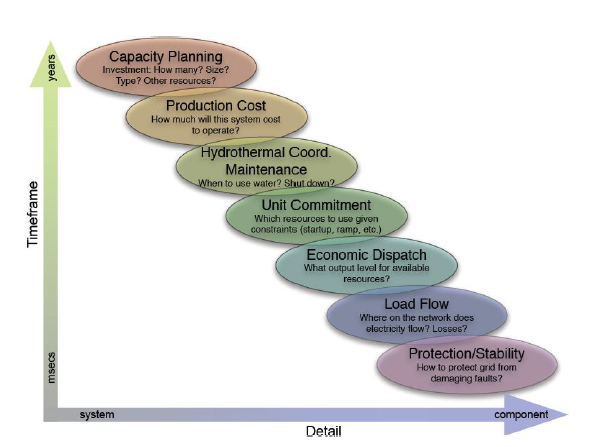
\includegraphics[scale=1]{anexos/hor-plan}
\par\end{centering}

\caption{\label{fig:Horizontes-de-planejamento}Horizontes de planejamento}
\end{figure}



Uma vez definida a demanda a atender, devemos escolher qual tipo de
usina implantar. Existem diversos tipos, como eólica, hidrelétrica,
nuclear, termelétrica (a gás, a carvão), entre outras. Além das diferenças
regionais entre a disponibilidade dos recursos naturais, há ainda
diferenças nas relações entre o custo de investimento inicial e o
custo de geração da energia. Por exemplo, uma usina termelétrica possui
geralmente um custo inicial menor que uma hidrelétrica, porém o custo
de geração da segunda é menor. A melhor solução a ser adotada possivelmente
passa pela utilização de uma combinação de diversos tipos, alguns
com custo de geração baixo mas altos investimentos iniciais para estarem
sempre ligados, e outros com baixos investimos iniciais mas alto custo
de geração para cobrir picos de demanda. Outras variáveis importantes,
além do custo das usinas, são a sazonalidade dos recursos e o tempo
de inicialização e desligamento de uma usina. O custo da operação do sistema de energia, incluindo todas suas restrições, também deve ser determinado. Para isso, é necessário realizar
o planejamento operacional, que observa horizontes menores e inclui,
por exemplo, o despacho econômico das usinas e a gestão de recursos
hídricos. 


Pode-se perceber que existem muitas variáveis envolvidas, custos desconhecidos,
e incertezas dos mais diversos tipos que afetam o funcionamento do
sistema, como a situação política do oriente médio ou até mesmo o
fenômeno El Niño. Considerar todas as variáveis ao mesmo tempo para
definir as quantidades ótimas, em qualquer estágio do planejamento,
requer um esforço computacional imenso, além de saber utilizar modelos estatísticos e utilizar métodos de mensuração de risco. Isso torna o estudo de métodos
de otimização um pré-requisito essencial para fazer uma boa gestão
de qualquer empresa que opera no mercado de energia.

Mas no que se consiste exatamente o mercado de energia?

% \subsection{Mecanismo de mercado}

Assim como no país fictício citado anteriormente, em todos os países a implantação inicial
da rede elétrica foi coordenada pela mesma instituição:
no caso, o governo. Isso mudou quando o Chile implantou o primeiro mercado de energia, em 1972, em que empresas vendiam a energia produzida por elas para as distribuidoras, por um preço determinado pelo mercado. Até então, todas as etapas do diagrama apresentado acima eram controladas pelo estado.
Assim, ao invés de ter um processo físico coordenando quanto cada empresa produz, é possível coordenar as quantidades fornecidas através da definição dos preços.
Caso os preços definidos sejam bem calibrados e não haja imperfeições
de mercado, é possível mostrar que as usinas fornecerão energia na
quantidade necessária, tal como uma empresa verticalmente integrada
faria dando ordens de produção para suas subsidiárias. Assim, estabelece-se
a fundamentação teórica para a criação de um mercado de energia.

Tal mercado tem vantagens e desvantagens. O mercado cria um ambiente competitivo e inovador que a longo e médio prazo pode conquistar avanços tecnológicos relevantes. Entretanto, um mercado mal formulado pode levar a uma competição desenfreada que pode levar ao não cumprimento de contratos e à falta de energia. 

Um exemplo interessante é o caso dos EUA e do Canadá, que possuem uma abordagem mista com relação à adoção de mercados de energia, em que cada estado ou província pode ou não adotar um esquema de mercado de energia. Na figura \ref{fig:mercado-eua}, está indicado em cores diferentes os diferentes mercados de energia existentes. Aqueles que possuem cores fracas não implementaram um mercado de energia, sendo o estado ou a província o responsável por fazer o planejamento e informar a quantidade produzida por cada produtor. Historicamente, nos EUA os mercados foram sendo implantados em alguns estados e passaram a ser adotados pelos estados vizinhos (um deles, o grupo Midwest ISO, conseguiu avançar para o Canadá, na província de Manitoba), após ter havido sucesso em suas implementações.  

\begin{figure}
\begin{centering}
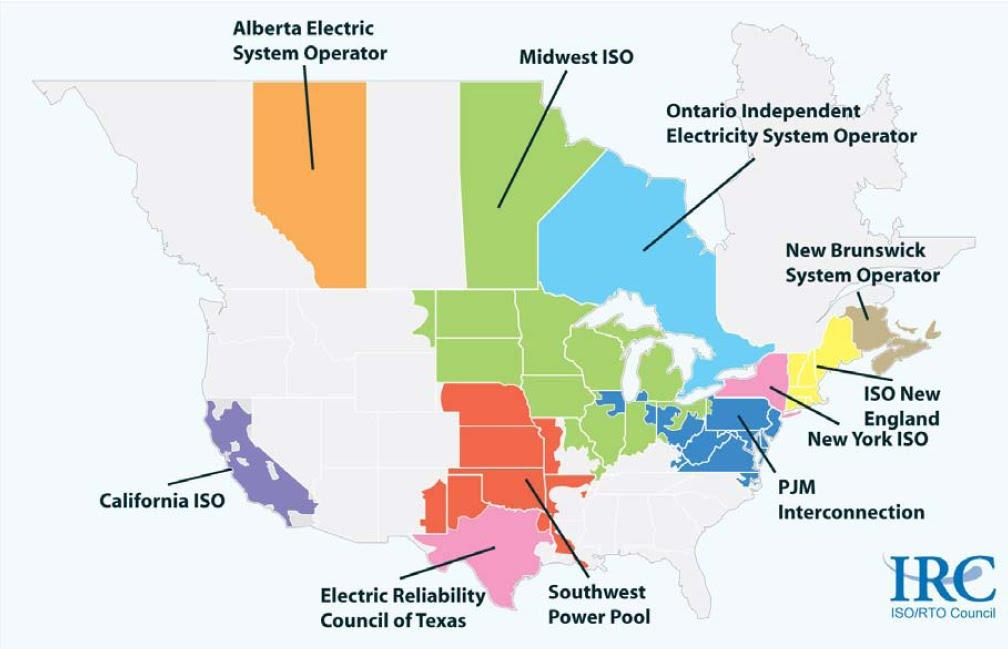
\includegraphics[scale=0.4]{anexos/mercados-eua.png}
\par\end{centering}

\caption{\label{fig:mercado-eua}A existência ou não de mercados de energia são definidos estado a estado nos EUA}
\end{figure}


Já as etapas de distribuição e transmissão são consideradas como monopólios
naturais. Entende-se por monopólio natural mercados que necessitam de
investimentos iniciais muito elevados e custos marginais muito baixos
e, com isso, a existência de concorrência poderia tornar impraticável
a existência de empresas que desejassem ofertar o serviço. Com isso,
é eficiente um esquema em que apenas uma empresa oferece o serviço
e este é regulamentada pelo governo. 

Faz parte do escopo deste trabalho, também, entender como oferecer os incentivos para que o mercado opere de forma eficiente. Se em um dado momento os atores não forem remunerados de forma adequado, gera-se um desincentivo para que novas empresas decidam entrar no negócio, diminuindo a competição e piorando a eficiência do mercado em médio prazo. 



%\subsection{Abertura do mercado no brasil}

\todo[inline]{incluir algo sobre a história da energia elétrica no brasil após a aula deste assunto}

O Brasil, assim como toda a América Latina, possui um alto percentual de usinas hidrelétricas em sua matriz energética. A figura \ref{fig:hidro-america-sul} mostra o percentual que essas usinas representam para cada país que possui mercado, assim como a existência ou não de um mercado de energia. 
Como mencionado anteriormente, a dependência de recursos hídricos (e de renováveis em geral) gera uma complexidade a mais para lidar quando planejamos o despacho das usinas. Para as usinas que possuem represa, é possível controlar seu estoque de água (até certo limite, claro) e decidir quando gerar energia com o que está no reservatório. No entanto, a quantidade de chuva em cada período é extremamente difícil de ser prevista. 
Podemos fazer decisões de consumo num período $t$ contando com chuva em $t+1$, mas se essa chuva não vir é possível que tenhamos que demandar uma alta quantia de energia de um tipo de usina mais custoso, como a termelétrica. Nesse e em outros casos, se faz necessária a mensuração do risco que corremos ao fazer decisões e não tomar decisões que possam colapsar o sistema com certa probabilidade. 


\begin{figure}[h]
\begin{centering}
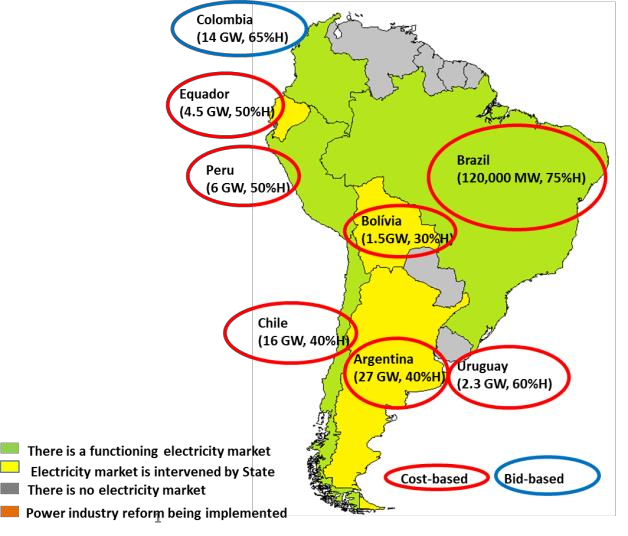
\includegraphics[scale=0.6]{anexos/hidro-america-sul.png}
\par\end{centering}

\caption{\label{fig:hidro-america-sul} Percentual de energia gerada por meio de usinas hidrelétricas e característica do mercado de energia por país}
\end{figure}


% Conclusão
Para realizar todas as atividades citadas acima, é preciso possuir
conhecimento de diversas áreas. A economia da energia elétrica é,
assim, um assunto multidisciplinar, que envolve disciplinas tão distintas
como economia, otimização, estatística, finanças e engenharia elétrica.
Uma visão global do processo de geração, assim como do funcionamento
do mercado de energia e sua interação com os consumidores, é exigida
do engenheiro elétrico do século XXI, não mais somente conhecimento
sobre capacitores e fluxos de potência. 



%%%%%%% OTIMIZAÇÃO %%%%%%%%%%%

\subsection{Revisão Otimização}
Esta sessão tem como objetivo apresentar os conceitos básicos de otimização que serão utilizados no decorrer do curso. Um modelo de otimização consiste em encontrar o valor máximo (mínimo) de uma \textbf{função objetivo}, por exemplo, o custo de geração de energia. Esta função possui um \textbf{vetor de variáveis de decisão} e é limitada por uma série de outras funções chamadas \textbf{restrições}.

Suponha que você é um dono de uma fábrica de móveis e deve decidir quais móveis produzir afim de obter o maior lucro possível. A fábrica produz armários e berços, que são representados pelas letras $A$ e $B$ respectivamente. No entanto, a quantidade produzida é limitada pelo estoque de matéria prima da fábrica, sendos estas madeira e ferro, representadas por $M$ e $F$. Sabemos que a receita líquida de um armário é de 4 reais e a do berço de 3 reais. Além disso, para se produzir um armário são necessárias 2 unidades de ferro e 1 unidade de madeira, e para o berço 1 unidade de ferro e 2 unidades de madeira. A fabrica possui 4 unidades de cada insumo em estoque. O problema pode se resumido em uma \textbf{matriz de tecnologia} apresentada na tabela \ref{tabela1}.

\begin{table}[H]
\begin{center}

\begin{tabular}{l|l|l|ll}
               & Armário & Berço & Estoque &  \\ \cline{1-4}
Ferro          & 2       & 1     & 4       &  \\ \cline{1-4}
Madeira        & 1       & 2     & 4       &  \\ \cline{1-4}
Lucro Marginal & 4       & 3     &         & 
\end{tabular}
\caption{Matriz de Tecnologia da Fábrica}
\label{tabela1}
\end{center}
\end{table}

Para encontrar o lucro ótimo devemos primeiro responder às seguintes perguntas:
\begin{itemize}
\item Quais são as variáveis de decisão do modelo?
\item Qual é a função objetivo do modelo?
\item Quais são as restrições do modelo?
\end{itemize}

A função objetivo é aquela que desejamos maximizar, no caso, o lucro. As variáveis de decisão são aquelas que devemos escolher afim de chegar ao resultado ótimo, ou seja, a quantidade produzida de cada móvel. As restrições do modelo são geradas pelas limitações do estoque. 

Formulação do problema:
\begin{itemize}
\item Variáveis de decisão: quantidade a produzir de cada produto $x_{A}$ e
$x_{B}$.
\item Função objetivo $f(x_{A},x_{B})=4x_{A}+3x_{B}$
\item Restrições:



\begin{itemize}
\item A quantidade de madeira utilizada não pode ser maior que o estoque:
$2x_{A}+1x_{B}\leq4$
\item A quantidade de ferro utilizada não pode ser maior que o estoque:
$1x_{A}+2x_{B}\leq4$
\item Não é permitido produzir quantidades negativas de armário ou berço: $x_{A}\geq0$ ,$x_{B}\geq0$\end{itemize}
\end{itemize}

Existe uma forma correta de escrever o problema acima com todas as suas informações. Em geral, é assim que você vai encontrar problemas de otimização e é assim que você deve procurar escreve-los. 

\begin{align}
    & \underset{x_A, x_B\geq0}{\text{maximizar}} \hspace{1cm} 4x_A+3x_B \label{eq1} \\
    & \text{s.a}  \hspace{2.2cm} 2x_A+x_B \leq 4; \label{eq2} \\
    &             \hspace{2.65cm} x_A+2x_B\leq 4, \label{eq3}
\end{align}

Em primeiro lugar temos a função objetivo, identificando se o problema é uma maximização ou uma minimização. É comum identificar o domínio das variáveis de decisão embaixo da palavra maximizar, neste caso, estamos dizendo que a quantidade produzida de cada móvel deve ser um número real não negativo. Entretanto, identificar o domínio e incluir as restrições $x_A, x_B \geq 0$ são exatamente a mesma coisa. 

Agora que já conhecemos o problema, temos que resolve-lo. Vamos colocar cada uma das restrições em um gráfico para entende-las melhor. 

\begin{figure}[H]
\begin{centering}
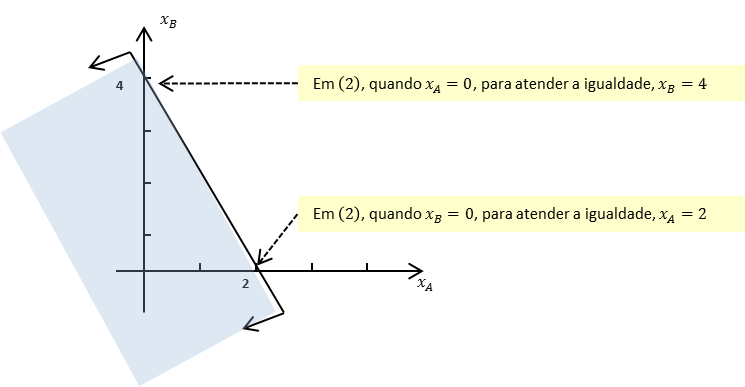
\includegraphics{pl1}\protect\caption{\label{fig:pl1}Gráfico equação (\ref{eq2})}
\end{centering}

\end{figure}

O que a figura \ref{fig:pl1} significa? No eixo $x$ temos a quantidade produzida de $x_A$ (armários), e no eixo $y$ a quantidade produzida de $x_B$ (berços). A reta desenhada na figura representa a restrição da equação \ref{eq2}. Todos os pontos a esquerda da reta são factíveis considerando apenas esta restrição. Como sabemos disso? Observe que pela restrição, se produzirmos apenas armários, a quantidade máxima produzida será 2 considerando as limitações de estoque, no caso dos berços, a quantidade será 4. Como a restrição é linear, e conheçemos dois pontos desta reta, basta ligar estes dois pontos para termos a representação gráfica da restrição.

De forma análoga, a figura \ref{fig:pl2} mostra a restrição escrita na equação \ref{eq3}.

\begin{figure}[H]
\begin{centering}
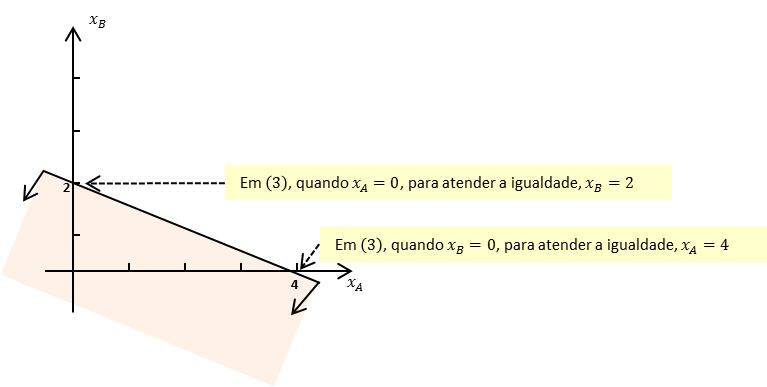
\includegraphics{pl2}\protect\caption{\label{fig:pl2}Gráfico equação (\ref{eq3})}
\end{centering}

\end{figure}

O conjunto de pontos viáveis pode ser encontrado combinando as duas figuras e levando em conta o domínio das variáveis de decisão. 

\begin{figure}[H]
\begin{centering}
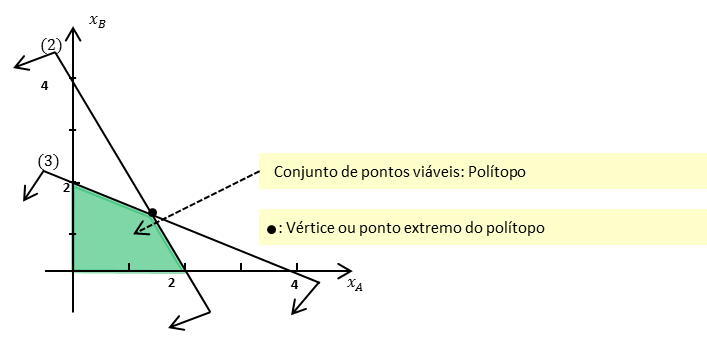
\includegraphics{pl3}\protect\caption{\label{fig:pl3}Gráfico conjunto de pontos viáveis}
\end{centering}

\end{figure}

Todos os pontos que estão na área verde da figura \ref{fig:pl3} são factíveis para a solução do nosso problema de otimização, porém apenas um deles é aquele que maximiza o lucro. Esta área é chamada de \textbf{poliedro}. Vamos encontrar qual o ponto ótimo utilizando o \textbf{gradiente}\footnote{Gradiente é o vetor das derivadas parciais da função objetivo.} da função objetivo para ver em qual direção que cresce mais rápido. Como se trata de uma função linear, o gradiente é constante e igual ao vetor $[4,3]$, representado na figura \ref{fig:pl4}.

\begin{figure}[H]
\begin{centering}
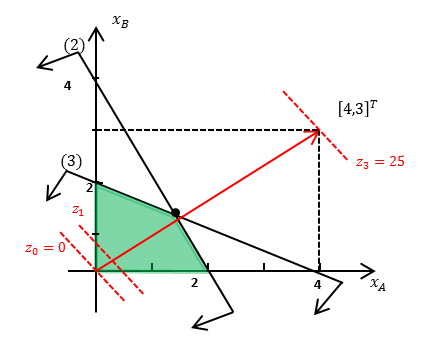
\includegraphics{pl4}\protect\caption{\label{fig:pl4}Gráfico curva de nível}
\end{centering}
\end{figure}

Com o gradiente podemos encontrar as \textbf{curvas de nível}, que são pontos onde a função objetivo tem o mesmo valor. As curvas de nível são perpendiculares ao vetor gradiente e também estão representadas na figura \ref{fig:pl4}. Finalmente, podemos resolver o problema caminhando com as curvas de nível para a direita até que ela chegue no último ponto dentro do poliedro dos pontos viáveis. 

\begin{figure}[H]
\begin{centering}
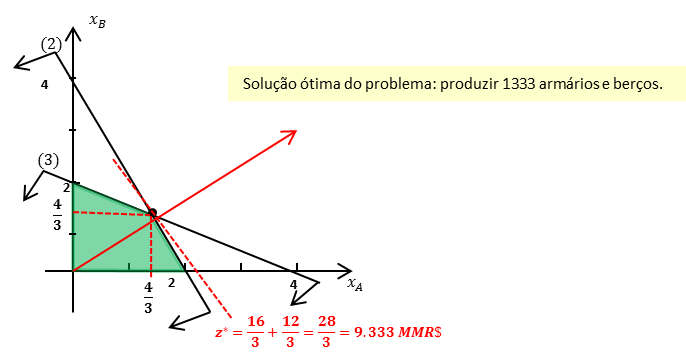
\includegraphics{pl5}\protect\caption{\label{fig:pl5}Gráfico solução ótima}
\end{centering}
\end{figure}

A figura \ref{fig:pl5} mostra a solução do problema. o Lúcro máximo é de $9.33$ reais e a solução ótima é aquela onde $x_A=x_B=\frac{4}{3}$.


Vamos colocar os passos para a resolução do problema de otimização acima em uma forma mais geral. Existem quatro passos básicos para se modelar um problema:
\begin{enumerate}
\item Compreensão do problema: 

\begin{itemize}
\item Identificar das partes relevantes o que se deseja tratar. Nesta parte,
geralmente são excluidas uma série de relações que não implicam em
uma direta, ou substancial, participação no objetivo do problema.
\end{itemize}
\item Identificação das variáveis de decisão: $x=[x_{1},...,x_{n}]^{T}$

\begin{itemize}
\item Quais são as variáveis que se deseja obter com a resolução do problema,
ou seja, o que se deseja encontrar (otimizar) e os seus respectivos
limites superiores e inferiores.
\end{itemize}
\item Identificar a função objetivo do problema: $f(x)$

\begin{itemize}
\item Especificar uma função que, dado uma possível configuração das variáveis
de decisão, reproduza o valor que se deseja maximixar ou minimixar
(otimizar): lucro, custo, confiabilidade, chance de se obter algum
resultado, distância de algum nível de referência,etc...
\end{itemize}
\item Identificar as condições que as variáveis devem atender: $g_{i}(x)\leq0$
para $i=1,...,m$

\begin{itemize}
\item Para serem válidas (viáveis) de serem escolhidas, através de inequação
ou equações.
\item É importante ressaltar que se uma possível solução não atender a alguma
das restrições, isso implica em descartar totalmente esta solução,
independentemente do valor da sua função objetivo. Logo, se existir
alguma possibilidade de discussão sobre o trade-off entre uma possível
violação e o valor da função objetivo, isso deve ser incoporado no
modelo.
\end{itemize}
\end{enumerate}

O problema do lucro ótimo da fábrica de móveis é uma \textbf{programação linear}, ou seja, tanto a função objetivo quanto as restrições são equações lineares. Todo problema de programação linear pode ser representado pela forma geral apresentada abaixo:

Forma compacta matricial
\begin{equation*}
\begin{aligned}
& \underset{x\geq0}{\text{maximizar}}
& & c^{T}x \\
& \text{s.a}
& & Ax \leq b.
\end{aligned}
\end{equation*}

Forma canônica,

\begin{equation*}
\begin{aligned}
& \underset{x}{\text{maximizar}}
& & \sum_{j=1}^{n}c_{j}\cdot x_{j} \\
& \text{s.a}
& &\sum_{j=1}^{n}a_{ij}\cdot x_{j}\leq b_{i},\qquad\forall i=1,...,m\\
& & & x_j \geq0\qquad\forall j=1,...,n.
\end{aligned}
\end{equation*}

Olhando para a forma matricial, $c$ são os coeficientes da função objetivo (4 e 3 no caso do exemplo da fábrida de móveis); $x$ são as variáveis de deicisão; $A$ é a matriz com os coeficientes das restrições; e $B$ representa o limite das restrições (no caso, o tamanho dos estoques). 
%\\

\textbf{\textit{Teoria da Dualidade}}

%\\

O \textbf{problema primal} é aquele problema que temos nas nossas mãos para resolver. Para obter algumas informações sobre o problema primal podemos utilizar o \textbf{problema dual}. No caso de uma máximização, o problema dual nos fornece um limite superior para o problema primal, se este limite superior for factível ele será o ótimo do problema primal. Isto pode ser reduzido em dois teoremas. 

\newtheorem{teo}{Teorema}[section]
\begin{teo}[Dualidade Forte]
Em um problema de programação linear, a solução ótima do problema primal será igual à solução ótima do problema dual se ambos forem viáveis. 
\end{teo}

\begin{teo}[Dualidade Fraca]
As soluções viáveis do problema dual são maiores ou iguais à solução do problema primal em um problema de maximização. No caso de um problema de minimização as relações são invertidas. 
\end{teo}


Voltando para o exemplo do problema de maximização do lucro da fábrica de móveis, lembre-se que ele era representado da seguinte forma:

\begin{align}
    & \underset{x\geq0}{\text{maximizar}} \hspace{1cm} 4x_A+3x_B \label{eq4} \\
    & \text{s.a}  \hspace{2.2cm} 2x_A+x_B \leq 4; \label{eq5} \\
    &             \hspace{2.65cm} x_A+2x_B\leq 4, \label{eq6}
\end{align}

Imagine que madeira e ferro estejam em falta no mercado, e que um comerciante deseja comprar o nosso estoque. Naturalmente, aceitaremos valores \todo{Revisar  valores de que}que, no total, sejam superiores ao nosso lucro fabricando os berços e armários. O problema do comerciante é minimizar o valor pago pelos nossos insumos levando em conta que nós só venderemos se o valor pago for maior do que o nosso lucro com a venda de berços e armários. As variáveis de decisão passam então a ser os preços dos insumos (madeira e ferro). O problema do comerciante é um problema dual do nosso problema de maximização do lucro. 

Vamos montar o problema do comerciante na forma de programação linear. A solução ótima do exemplo atende todas as restrições então, ao multiplicarmos a restrição \ref{eq4} por 3, obteremos a seguinte inequação, válida para todos os pontos viáveis.

\begin{equation}
6x_{A}+3x_{B}\leq12
\label{eq:dual1}
\end{equation}

Todos os coeficientes da desigualdade acima são maiores ou iguais do que seus respectivos coeficientes na função objetivo do problema de máximização de lucro, portanto o lucro será sempre menor do que 12.

Se fizermos uma combinação linear positiva das restrições (\ref{eq4}) e (\ref{eq5}), multiplicando-as pelo preço de cada insumo, representados por $y_A$ e $y_B$, a desigualdade será valida para todos os pontos que atendem às restrições originais:

\begin{table}[h]
\begin{center}
\begin{tabular}{lllll}
 & $y_{A}\cdot(2\cdot x_{A}+1\cdot x_{B})\leq y_{A}\cdot4$
 &  &  &  \\
 & $y_{B}\cdot(1\cdot x_{A}+2\cdot x_{B})\leq y_{B}\cdot4$ \hspace{1.0cm} + &  &  &  \\ \cline{2-2}
 & $(y_{A}\cdot2+y_{B}\cdot1)\cdot x_{A}+(y_{A}\cdot1+y_{B}\cdot2)\cdot x_{B}\leq y_{A}\cdot4+y_{B}\cdot4$ &  &  & 
 &   &  & % & 
\end{tabular}
\end{center}
\end{table}

Assumindo os valores $y_{A}=5/3$ e $y_{B}=2/3$, por exemplo, obteremos um
limite superior igual a $28/3$ , que sabemos ser o máximo do problema
da maximização do lucro. Isso nos mostra que o limite superior obtido por essa
escolha de multiplicadores resulta no menor limite possível, ou seja
, o limite ótimo. O teorema da dualidade forte garante que o GAP (diferença entre a solução dual e a primal) em problemas de otimização linear será sempre zero. Olhando para a figura \ref{fig:dualgap}

\begin{figure}[H]
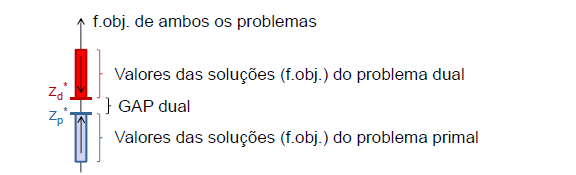
\includegraphics{pl6}\protect\caption{GAP dual}
\label{fig:dualgap}
\end{figure}


Retornando a resolução do problema em $y_{i},$ como podemos gerar
uma sistemática para encontrar os pesos de maneira que eles proporcionem
o menor limite superior (mínimo)?

Será necessário impor que cada coeficiente\footnote{Entenda como coeficiente toda a expressão que multiplica $x_A$ ou $x_B$.} da desigualdade encontrada
seja superior ao respectivo coeficiente da função objetivo : $z_{p}=4\cdot x_{A}+3x_{B}$

\begin{equation}
y_{A}\cdot2+y_{B}\cdot1\geq4
\end{equation}

\begin{equation}
y_{A}\cdot1+y_{B}\cdot2\geq3
\end{equation}

Com isso, o lado direito dessa nova desigualdade será sempre maior
que qualquer valor que a função objetivo possa valer dentro do conjunto
de pontos viáveis:

\begin{equation}
4\cdot x_{A}+3x_{B}\leq(y_{A}\cdot2+y_{B}\cdot1)\cdot x_{A}+(y_{A}\cdot1+y_{B}\cdot2)x_{B}\leq y_{A}\cdot4+y_{B}\cdot4
\end{equation}

Assim, queremos minimizar o limite superior, mexendo nos multiplicadores
$y_{i}$, sujeita a esses multiplicadores gerarem um limite superior:

\begin{align}
    & \underset{y\geq0}{\text{minimizar}} \hspace{1cm} 4y_A+4y_B \label{eq6} \\
    & \text{s.a}  \hspace{2.2cm} 2y_A+y_B \geq 4; \label{eq7} \\
    &             \hspace{2.65cm} y_A+2y_B\geq 3, \label{eq8}
\end{align}

O problema acima é um problema dual da programação linear da maximização do lucro. Ao mesmo tempo, ele é o problema do comerciante que deseja comprar nosso estoque. Ao solucionar o problema do comerciante (dual) encontramos os preços pelos quais seriamos indiferentes entre produzir móveis ou vender insumos. A figura \ref{pldual1} mostra a solução do problema dual de forma análoga à que fizemos para o problema primal. 

\begin{figure}[H]
\begin{centering}
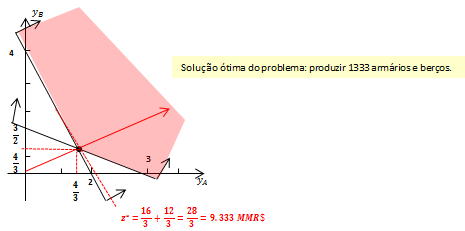
\includegraphics{pldual1}\protect\caption{\label{pldual1}Solução do problema dual}
\end{centering}
\end{figure}


De forma geral, um problema de programação linear definido como: 

\begin{equation*}
\begin{aligned}
& \underset{x\geq0}{\text{maximizar}}
& & c^{T}x \\
& \text{s.a}
& & Ax \leq b.
\end{aligned}
\end{equation*}

Tem a seguinte representação dual:

\begin{equation*}
\begin{aligned}
& \underset{y\geq0}{\text{minimizar}}
& & y^{T}b \\
& \text{s.a}
& & Ay^{T} \geq c.
\end{aligned}
\end{equation*}


\subsection{Revisão Estatística}

Otimização e estatística caminham juntas, principalmente quando estamos resolvendo problemas mais complexos. Imagine que queremos modelar um contrato de um parque eólico no ambiente livre (ACL). Para determinar o contrato, precisamos de projeções futuras da velocidade do vento, da potência gerada pelo parque e do preço da energia. Em outras palavras, precisamos gerar vários cenários possíveis para o futuro, e fazemos isto utilizando conceitos de estatística e de probabilidade. 

Como não sabemos o que vai acontecer no futuro, nossos cenários de possíveis realizações resultam em \textbf{distribuições de probabilidade}, e precisamos conhecer bem as características destas distribuições para construir cenários coerentes com a realidade. Uma distribuição de probabilidade descreve as chances de uma determinada variável assumir diferentes valores. Em outras palavras, uma distribuição é uma função que transforma valores de uma variável em probabilidade. 

Suponha que estamos jogando uma moeda. Os resultados possíveis são cara e coroa, se representarmos cara pelo número 1, e coroa por 0, temos o domínio de uma distribuição de probabilidade. A distribuição da moeda nos dirá que em $50\%$ das vezes o resultado será cara, e em $50\%$ será coroa. Esta distribuição é conhecida como \textit{distribuição de Bernoulli}.

A distribuição de Bernoulli é uma \textbf{distribuição discreta}. Em muitos casos pode ser interessante representar uma variável por uma \textbf{distribuição contínua}, ou seja, uma variável que pode assumir qualquer valor em um intervalo. A mais importante das distribuições contínuas é a \textbf{distribuição normal}. 
\\

\textbf{\textit{Distribuições Discretas}}


Já vimos que uma moeda pode ser caracterizada como uma distribuição discreta. Suponha agora que estamos jogando um dado. Ele pode assumir valores de 1 a 6 em intervalos discretos, ou seja, apenas os números inteiros de 1 a 6. A figura \ref{fig:prob1} apresenta o \textbf{histograma} de um dado. 

\begin{figure}[H]
\begin{centering}
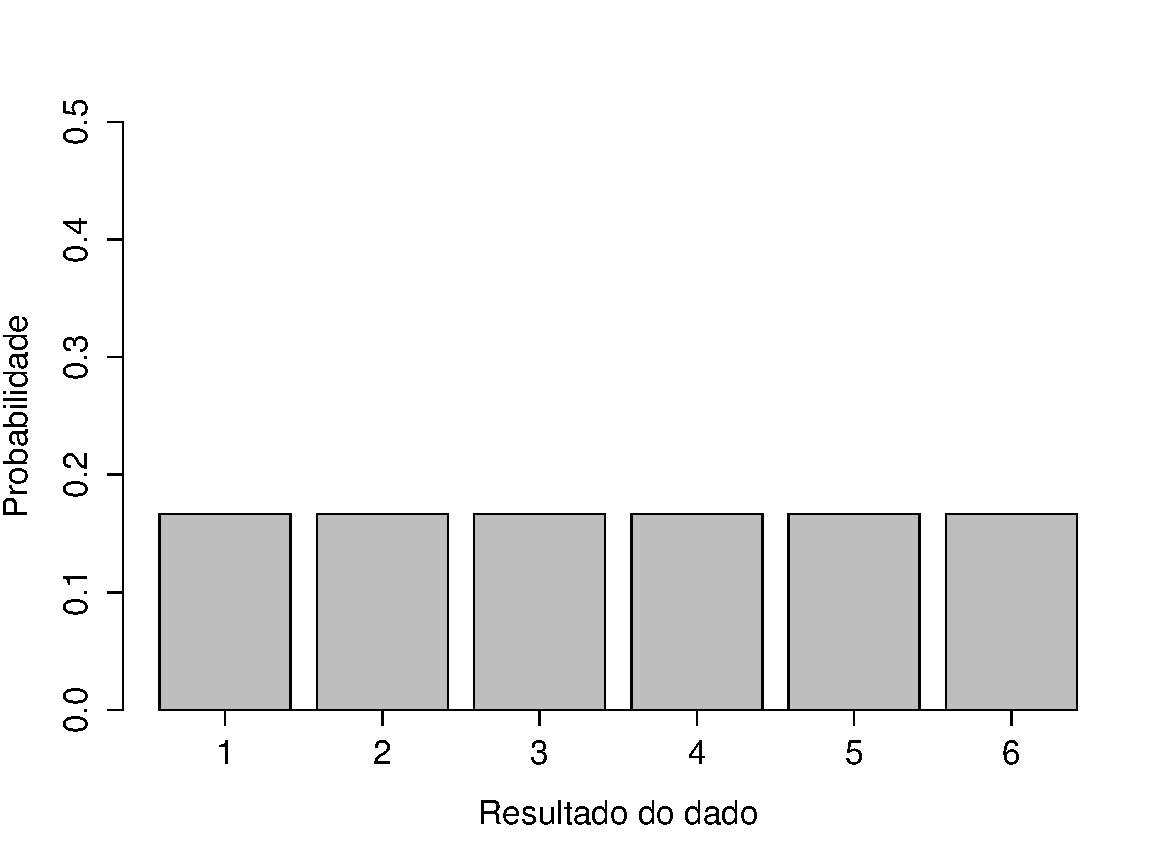
\includegraphics[scale=0.5]{uniforme-discreta}\protect\caption{\label{fig:prob1}Histograma de um dado}
\end{centering}
\end{figure}

No eixo $x$ temos os possíveis resultados do dado, ou seja, inteiros de 1 até 6. No eixo $y$ temos a probabilidade de cada resultado igual a $\frac{1}{6}$. Esta é uma \textbf{distribuição uniforme discreta}. O histograma apresenta os valores da variável no eixo $x$ e a probabilidade no eixo $y$. Entretanto, pode ser interessante olhar para a distribuição de probabilidade em sua forma acumulada, e não na forma de densidade como no histograma. 

\begin{figure}[H]
\begin{centering}
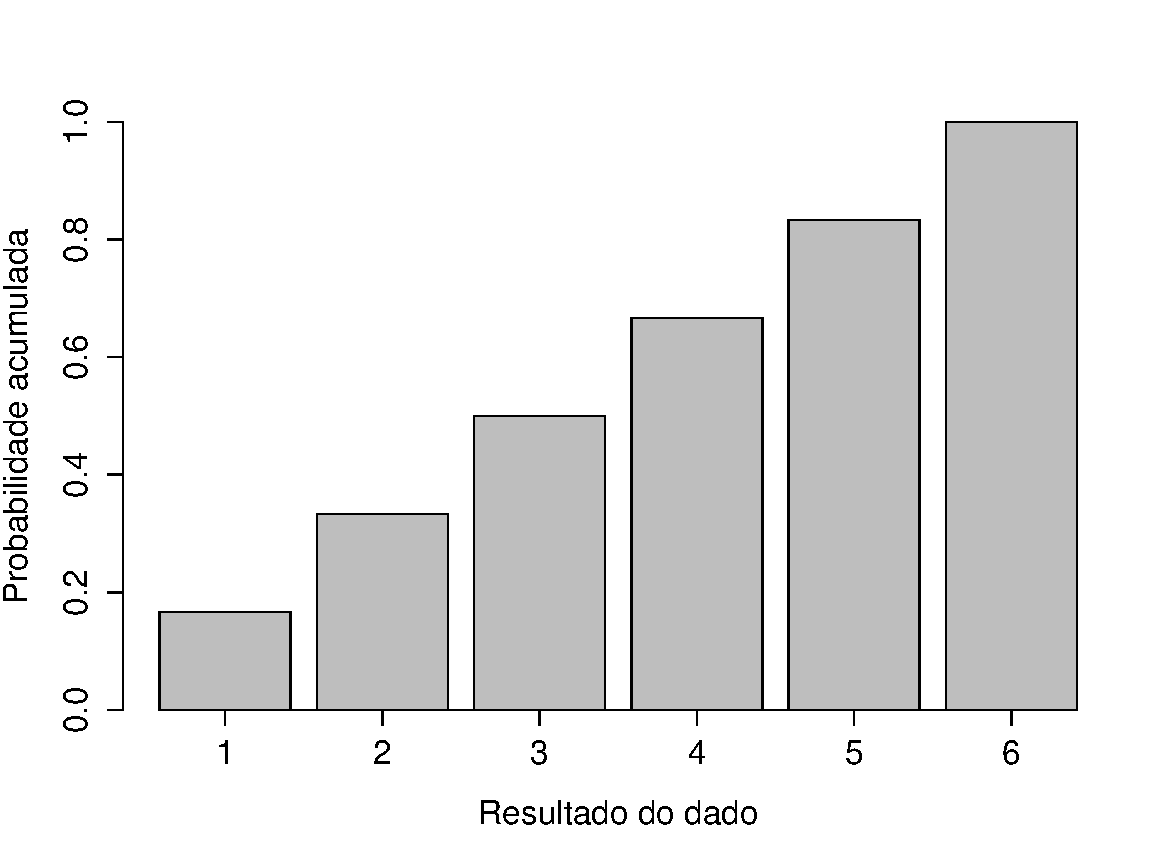
\includegraphics[scale=0.5]{uniforme-discreta-acumulada}\protect\caption{\label{fig:prob2}Distribuição acumulada de um dado}
\end{centering}
\end{figure}

A figura \ref{fig:prob2} mostra a mesma distribuição da figura \ref{fig:prob1}, porém em sua forma acumulada. No caso, a função acumulada em 4, por exemplo, representa a probabilidade de tirarmos um número menor ou igual a 4 no dado, $p(x\leq4)$. Observe que a distribuição acumulada termina onde a probabilidade assume o valor 1, ou $100\%$. Isto é o mesmo que dizer que com $100\%$ de chance tiraremos um número menor ou igual a 6 no dado, o que é verdade. No caso discreto, a distribuição acumulada terá sempre esta forma de escada, e o histograma poderá ser representado na forma de barras (fig. \ref{fig:prob1}).


Podemos escrever a distribuição do dado como uma fórmula matemática, no caso da densidade:

\begin{equation}
f(x)=p(x)=\frac{1}{6},~~~x\in [1,2,3,4,5,6]
\end{equation}

No caso da função acumulada:

\begin{equation}
F(x)=p(X\leq x)=\frac{1}{6}x,~~~x\in [1,2,3,4,5,6]
\end{equation}

Por convensão, usamos $f$ minúsculo para a função densidade e $F$ maiúsculo para a função acumulada. Além disso, o $X$ maiúsculo representa a variável aleatória do dado, e o $x$ minúsculo representa uma realização da mesma. Podemos escrever $p(X\leq 3)=\frac{1}{2}$, por exemplo. 

Por último, é interessante calcular a média e a variância das distribuições de probabilidade. A média é uma medida de \textbf{tendência central} e a variância mede a \textbf{dispersão} em torno da média. 

\begin{itemize}
\item média $=E[X]=\sum_{i=1}^n p_i x_i$
\item variância $=\sigma^2(X)=\sum_{i=1}^n p_i (x_i-E[X])^2$
\end{itemize}

onde, $p_i$ é a probabilidade do resultado $i$ acontecer. No caso da distribuição do dado esta probabilidade é igual a $\frac{1}{6}$ para todo $i$.

No caso do dado, a média e a variância são iguais a $3.5$ e $2.9$ respectivamente. Entretanto, a variância é uma medida difícil de interpretar. Imagine que estamos diante de uma distribuição de potência, a variância será medida então em potência ao quadrado. Para voltarmos para potência basta calcular o \textbf{desvio padrão}, que é a raiz quadrada da variância.\\



\textbf{\textit{Distribuições Continuas}}

Uma distribuição é contínua se seu domínio for contínuo. A mais conhecida das distribuições contínuas é a distribuição normal, seu histograma é apresentado na figura \ref{fig:prob3} e sua distribuição acumulada na figura \ref{fig:prob4}. 


\begin{figure}[H]
\begin{centering}
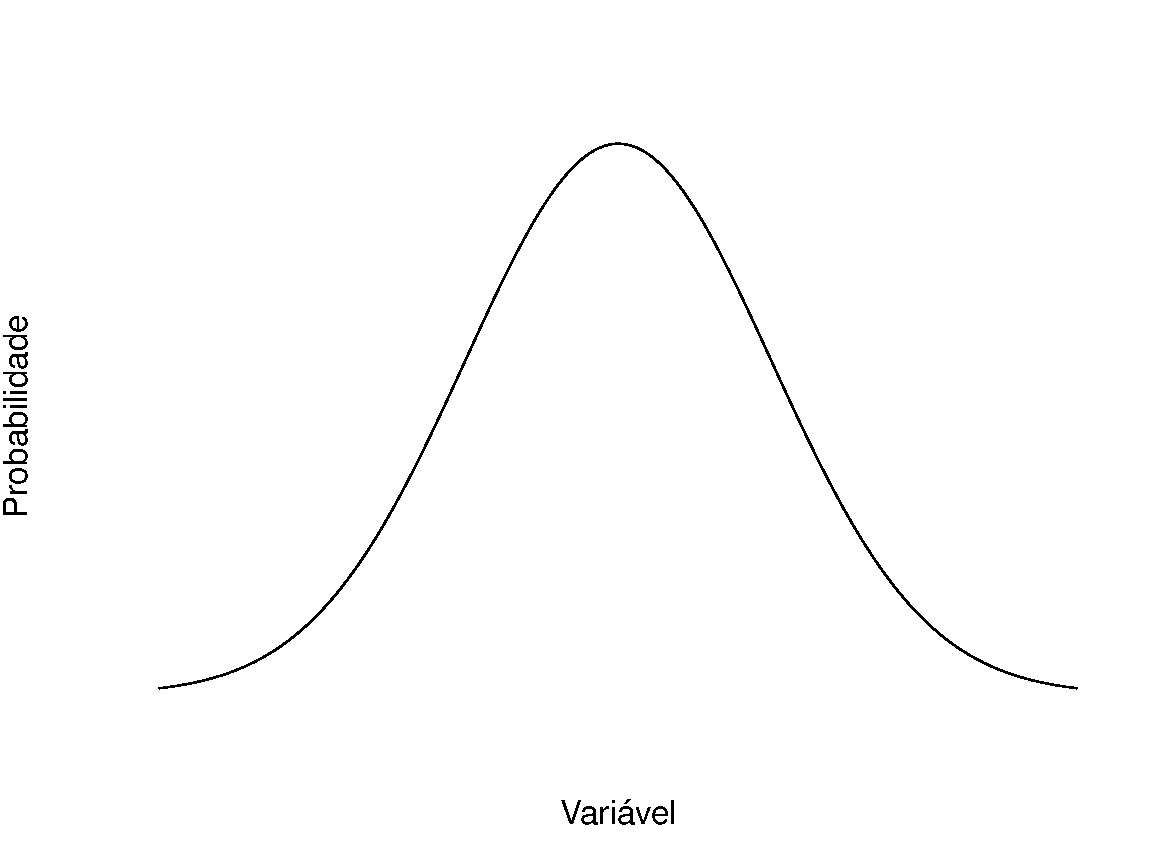
\includegraphics[scale=0.5]{histograma-normal}\protect\caption{\label{fig:prob3}Distribuição normal}
\end{centering}
\end{figure}

\begin{figure}[H]
\begin{centering}
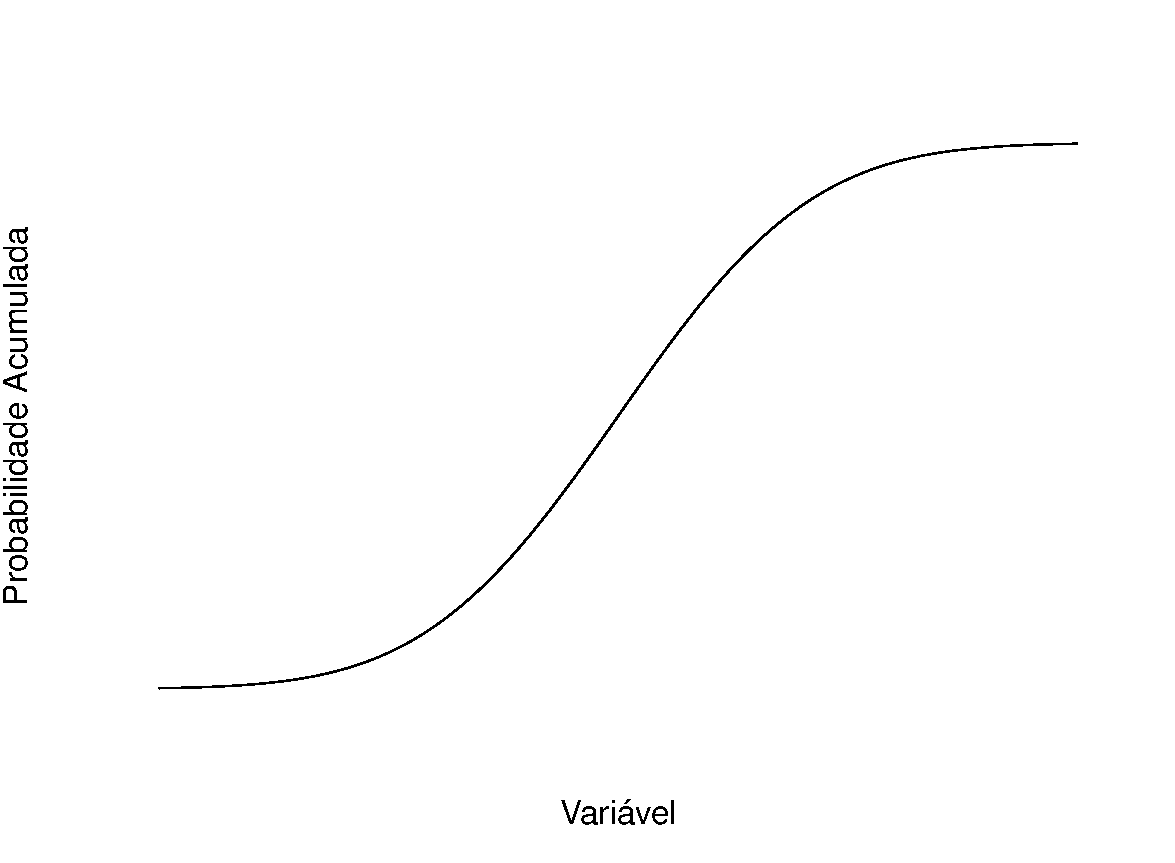
\includegraphics[scale=0.5]{histograma-normal-acumulada}\protect\caption{\label{fig:prob4}Distribuição normal acumulada}
\end{centering}
\end{figure}

O histograma de uma distribuição contínua não pode mais ser desenhado na forma de barras, e a distribuição acumulada não terá mais a forma de escada. Entretanto, a interpretação é muito semelhante à do caso discreto. Como uma distribuição contínua tem infinitos pontos no domínio, falar da probabilidade de ocorrência de um ponto isolado perde o sentido, pois esta probabilidade será igual a zero. O mais usual é falar da probabilidade de intervalos, por exemplo, a probabilidade de $x$ estar entre 1 e 2. 

Assim como no caso discreto, podemos representar as distribuições contínuas com uma fórmula, no caso da normal:

\begin{equation}
f(x)=\frac{1}{\sqrt{2 \pi \sigma^2}} e^{-\frac{(x-\mu)^2}{2\sigma^2}}
\end{equation}

A fórmula da distribuição acumulada da normal não é conhecida, entretanto, ela já foi toda tabelada e podemos utiliza-la sem problemas. Observe que na fórmula da normal temos os parâmetros $\mu$ e $\sigma^2$, que são respectivamente a média e a variância da distribuição. Portanto, se uma certa variável é normal e conhecemos sua média e sua variância, conhecemos também toda a distribuição desta variável.

Para calcular a média e a variância de uma distribuição contínua temos que calcular uma soma de infinitos elementos, por isto, o somatório é substituido pela integral.

\begin{itemize}
\item média $=\mu_X =E[X]=\int_{-\infty}^{\infty} xf(x)dx$
\item variância $=\sigma^2_X=\int_{-\infty}^{\infty} (x-E[X])^2 f(x)dx$  \end{itemize}
%\\

\textbf{\textit{Quantis}}

Uma fórma interessante de olhar para uma distribuição é separando-a em \textbf{quantis}. Quantis são pontos no domínio da distribuição acumulada que separam a mesma em intervalos iguais. Por exemplo, suponha que dividimos uma distribuição em quatro quantis\footnote{A divisão em quatro quantis é conhecida como quartil.}, a probabilidade de um elemento do domínio estar em um destes quantis é de $25\%$, e um mesmo elemento nunca estará em dois quantis ao mesmo tempo. 

Para ilustrar, suponha uma distribuição que assume os valores inteiros $[1,1,4,6,7,11,12,12]$. O primeiro quantil será $[1,1]$; o segundo será $[4,6]$, o terceiro será $[7,11]$ e o quarto será $[12,12]$. O segundo quartil, também chamado de mediana, divide a amostra no meio. A mediana é uma medida de tendência central assim como a média.

Quantis são muito úteis quando queremos estudar partes separadas das distribuições. Imagine uma distribuição de geração de um parque eólico, se queremos ver quais são os $5\%$ piores cenários de geração do nosso parque, basta separar a distribuição em 100 quantis e pegar os primeiros 5.

\section{Aula 2}

\subsection{História da Energia Elétrica}


\subsubsection{Evolução da energia elétrica}

Este capítulo contará um pouco sobre a história da energia elétrica e como chegamos aonde estamos, partindo da invenção da lâmpada para complexos sistemas elétricos. A tablela \ref{linha-tempo} mostra um pouco desta história.

A primeira invenção que teve utilidade direta para as pessoas comuns foi feita em 1752 por Benjamin Franklin. O para raios foi o primeiro passo para o domínio da energia elétrica pelo homem. A partir daí as descobertas vieram cada vez mais rápido, e avanços teóricos permitiram o conhecimento das leis fundamentais da energia elétrica, como a lei de Ohm, que cria a relação entre corrente, tensão e resistência elétrica.

Estas descobertas culminaram na invenção da lçampada por Thomas Edison e posteriormente levaram ao conhecimento do elétron, que foi descoberto por J. J. Thomson. No entanto, ainda existiam grandes obstáculos para a popularização da energia elétrica. Os primeiros sistemas eram locais, e não havia qualquer tipo de conexão entre eles. Um fato curioso é que as pessoas não pagavam pelo consumo de energia, e sim pelas lâmpadas. 


\begin{table}[H]
\caption{\label{linha-tempo}Linha do tempo da energia elétrica}
\centering
\begin{minipage}[H]{.8\linewidth}
\color{gray}
\rule{\linewidth}{0.9pt}
\ytl{Pré-1700}{Até o século XVIII, estudos empíricos indicavam a existência de elementos
associados a eletricidade em experiências feitas com animais e elementos químicos} 
\ytl{1733}{Du Fay (Francês) publica a existência de dois tipos de eletricidade, o que
mais tarde seria identificado como "positivo" e "negativo". Ele também identifica a
diferença entre isolantes e condutores} 
\ytl{1752}{Benjamim Franklin, a partir de suas observações sobre descargas
atmosféricas, Franklin inventa o pára-raios}
\ytl{1800}{O conde Alessandro Volta desenvolve a pilha voltaica, precursora das
baterias modernas. A pilha de Volta era capaz de produzir corrente continua}
\ytl{1826}{André-Marie Ampere mostra que uma corrente elétrica apresenta uma
expressão que relaciona a corrente elétrica com a produção de um campo magnético}
\ytl{1827}{A lei de Ohm relaciona as grandezas fundamentais da
eletricidade: tensão, corrente e resistência elétrica}
\ytl{1832}{Faraday mostra como a variação do campo magnético pode gerar uma
corrente elétrica. 
Paralelamente, Gauss estabelece a relação entre carga elétrica dentro de uma
superfície de volume limitado e o campo elétrico que passa através de uma
superfície}
\ytl{1850}{James Clerk Maxwell encerra um ciclo da história da eletricidade ao formular as
equações que unificam a descrição dos comportamentos elétrico e magnético da
matéria. Esta é a teoria que surge juntando a lei de Ampere, a lei de Gauss e a lei de
Faraday}
\ytl{1873}{O cientista belga Zénobe Gramme demonstrou que a eletricidade
podia ser transmitida de um ponto a outro através de cabos condutores aéreos}
\ytl{1879}{Thomas Edison inventa a lâmpada incandescente. Dois anos depois
constrói na cidade de Nova York a primeira central de energia elétrica com
sistema de distribuição. Nesta época, o serviço de energia elétrica era vendido por lâmpadas, não
eletricidade}
\ytl{1890}{O descobrimento do elétron por Joseph John Thomson, na década de 1890 pode ser
considerado o marco da passagem da ciência da eletricidade para a da eletrônica, que
proporcionou um avanço tecnológico ainda mais acelerado}
\bigskip
\rule{\linewidth}{1pt}%
\end{minipage}%
\end{table}

\subsubsection{Guerra das correntes}

Um dos primeiros grandes debates na história da energia elétrica foi aquele conhecido como a Guerra das Correntes. De um lado estava Thomas
Edison ,com o financiamento do J.P Morgan, que propunha utilizar um
sistema de \textbf{corrente continua} para atender localmente as cidades; do outro lado estava Nicolas
Tesla, com o patrocínio de George Westinghouse, que propôs que
os sistemas elétricos deveriam se expandir a partir do que eles chamavam
de \textbf{corrente alternada}. 

Vamos entender o que são essas correntes. A corrente contínua é aquela onde existe um fluxo ordenado de elétrons sempre na mesma direção. Nos dias de hoje, este tipo de corrente é utilizado em baterias na maioria dos aparelhos eletrônicos portáteis que carregamos, como tablets, celulares, etc. Sempre que você ver algum aparelho elétrico com polo positivo e polo negativo, você estará lidando com corrente contínua. A corrente alternada, por outro lado, é aquela onde o sentido dos elétrons varia no tempo, em geral, na forma \textbf{senoidal}, ou seja, como ondas. A corrente que sai da nossa casa no Brasil é alternada, é por isso que nossos aparelhos eletrônicos possuem uma fonte. 

A ideia da corrente alternada seria diminuir as perdas elétricas com um aumento da tensão e uma redução da corrente. Edison argumentava que este tipo de aumento poderia ser perigoso.


% Figura corrente alternada
\begin{figure}[H]
\begin{center}
\fbox {
    \begin{tikzpicture}[domain=0:4]
        \draw[very thin,color=gray] (-0.1,-2.1) grid (3.9,2.1);
        \draw[->] (-0.2,0) -- (4.2,0) node[right] {$t$};
        \draw[->] (0,-2.2) -- (0,2.2) node[above] {$V$};
        \draw[smooth, color=blue] plot[id=sin] function{sin(5*x)} 
            node[right] {Corrente alternada};
    \end{tikzpicture}1
    }
\caption{\label{fig:corrente-alternada} Característica da corrente alternada}
\end{center}
\end{figure}




% Figura corrente contínua
\begin{figure}[H]
\begin{center}
\fbox {
    \begin{tikzpicture}[domain=0:4]
        \draw[very thin,color=gray] (-0.1,-0.1) grid (3.9,3.9);
        \draw[->] (-0.2,0) -- (4.2,0) node[right] {$i$};
        \draw[->] (0,-0.2) -- (0,4.2) node[above] {$V$};
        \draw[smooth, color=blue] plot[id=sin] function{2} 
            node[right] {Corrente contínua};
    \end{tikzpicture}
    }
\caption{\label{fig:corrente-continua}Característica da corrente contínua}
\end{center}
\end{figure}


Quem venceu a Guerra das Correntes foi a corrente alternada, no entanto, se a guerra fosse hoje, Edison teria mais argumentos, pois naquela época o único aparelho elétrico alimentado pelas correntes eram as lâmpadas.
.Hoje, como mencionado anteriormente, alguns equipamentos utilizam corrente contínua por exemplo:
celular, MP3 player e computador.

A guerra parece não ter terminado, além dos aparelhos que utilizam corrente contínua, estão surgindo formas de geração de energia, como painéis solares, que geram neste tipo de corrente. Painéis solares estão cada vez mais modernos e baratos, e em alguns países as pessoas já estão começado a utiliza-los em casa. Acredite se quiser, já existe até um mercado de aluguel de telhados, onde empresas pagam para colocar painéis em cima da sua casa. Apesar do mercado de energia solar brasileiro ainda ser muito pequeno, já existem geradores privados, como shopping centers que possuem muito espaço para colocar os painéis. 

As linhas de corrente contínua tem custo inicial muito alto, mas conforme a linha cresce este custo começa a ser diluído, pois uma vez instalada, aumenta-la é barato. As linhas de corrente contínua, por outro lado, possuem um custo inicial barato dado que as grande maioria dos geradores já geram em corrente contínua. Entretanto, aumentar a linha vai ficando cada vez mais caro. Em um país com as dimensões do Brasil vale a pena considerar a construção de linhas de corrente contínua, inclusive, uma linha está sendo construída ligando a região norte á região sudeste. 

\begin{figure}[H]
\begin{centering}
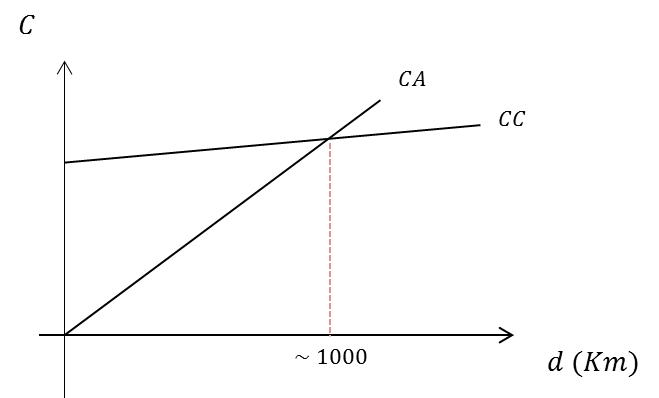
\includegraphics{aula2_3}\protect\caption{\label{fig:aula2_3} Corrente contínua e Corrente alternada }
\end{centering}

\end{figure}

\subsubsection{Sistemas elétricos em corrente alternada}

No sécilo XIX, o cientista ingês M. Faraday realizou o seguinte experimento: ele pegou uma pilha ,adicionou um chave para ligar e desligar essa pilha e colocou uma bobina com fios enrolados, fechando um circuito; do outro lado Faraday colocou um aparelho conhecido com galvanômetro, que tem a capacidade de detectar correntes elétricas, em um circuito fechado sem ligação com aquele da pilha. Então, a chave que estava aberta foi fechada, e o galvanômetro captou uma corrente mesmo estando em outro circuito. Faraday percebeu que o que levava à reação do galvanômetro era o fluxo magnético que conectava com o outro lado do experimento gerava uma corrente. Um ponto relevante no experimento é que Faraday sabia que a corrente provocava fluxo mas não sabia que fluxo provocava corrente. Então esse equipamento movia quando a chave era virada porem depois o equipamento voltava a posição inicial. Quando era desligada a chave, as linhas de fluxos desapareciam e o outro equipamento movia para o outro lado. Assim, quando era ligado o equipamento movimentava-se para um lado e quando desligado o movimento era contrário, invertendo assim o sentido (Figura \ref{fig:aula2_4}). 
\begin{figure}[H]
\begin{centering}
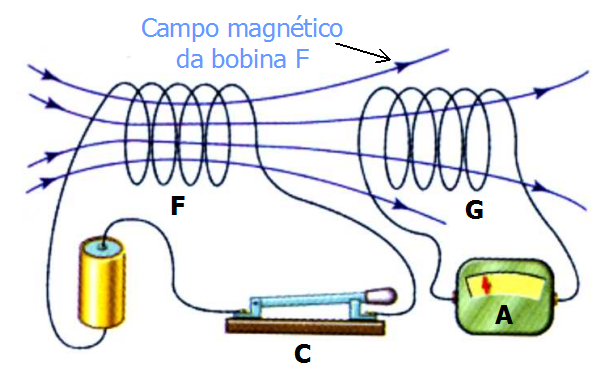
\includegraphics{aula2_4}\protect\caption{\label{fig:aula2_4}Experimento de M.Faraday }
\end{centering}

\end{figure}
Quem explicou e formalizou o experimento de Faraday foi Lenz, que descobriu a lei que levou o seu nome. A lei de Lenz postula que o sentido da corrente é o oposto da variação do campo magnético que lhe deu origem. O
experimento de Lenz é semelhante ao de Faraday, no entanto ele utilizou um imã para produzir as correntes de produzir linhas de fluxos provocados por correntes. Lenz injetou um campo magnético na espira, ou seja aproximou
o imã da espira e observou que quando aproxima o imã da espira
apareciam linhas de campo de sentido contrário ao movimento que foi
imposto. A medida que ele aproximava mais o imã apareciam linhas de campo no
sentido contrário, que induziam a passagem de corrente
elétrica nessa espira para recuperar o equilíbrio \ref{fig:aula2_5}. Assim,
Lenz (1834) respondeu porque a corrente elétrica mudava de sentido
quando se retirava o campo magnético.
\begin{figure}[H]
\begin{centering}
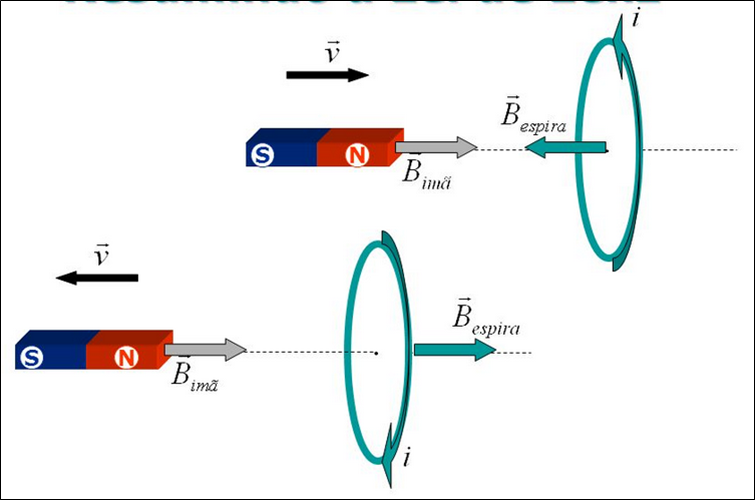
\includegraphics{aula2_5}\protect\caption{\label{fig:aula2_5}Experimento de Lenz }
\end{centering}

\end{figure}

A grandeza escalar que mede o número de linhas de indução que atravessam
a área \textit{\textcolor{black}{A }}de uma espira imersa num campo
magnético uniforme \ref{fig:aula2_6} é chamada fluxo magnético $(\Phi)$, sendo definida
por:
\begin{equation}\label{eq:fluxomag}
\Phi=n\cdot B\cdot A\cdot\cos\theta 
\end{equation}


onde,

$A$- área em $m^{2}$

$B$- campo magnético em tesla $(T)$

$\Phi$- fluxo magnético em weber $(Wb)$

$n$- número de espiras.




\begin{figure}[H]
\begin{centering}
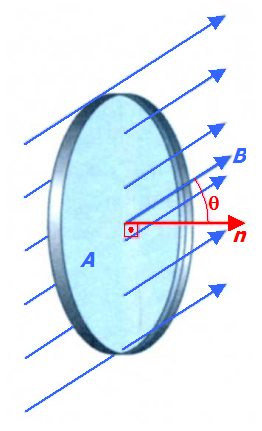
\includegraphics{aula2_6}\protect\caption{\label{fig:aula2_6}Fluxo magnético }
\end{centering}

\end{figure}
Assim, o fluxo magnético será proporcional ao número de espiras, a
intensidade das linhas de campos, a área da seção e oo cosseno de $\Theta$
(o angulo entre as linhas de campo magnético e a linha perpendicular
a espira). 
Por exemplo quando $\Theta=0$,fluxo máximo,$\cos\Theta=1$, então
$\Phi=n\cdot B\cdot A$ (Figura \ref{fig:aula2_7}); e quando $\Theta=90^{\circ}$,sem fluxos,$\cos\Theta=0$,
então $\Phi=0$ (Figura \ref{fig:aula2_8}).

\begin{figure}[H]
\begin{centering}
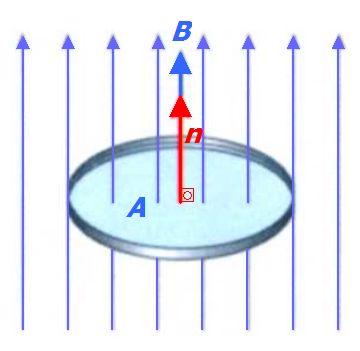
\includegraphics{aula2_7}\protect\caption{\label{fig:aula2_7}Fluxo máximo }
\end{centering}

\end{figure}
\begin{figure}[H]
\begin{centering}
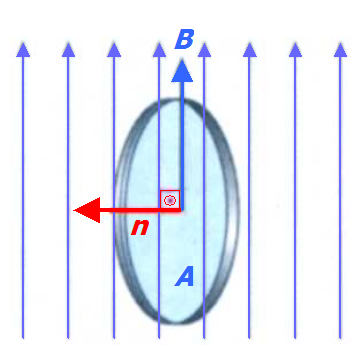
\includegraphics{aula2_8}\protect\caption{\label{fig:aula2_8}Sem fluxo }
\end{centering}

\end{figure}

O outro experimento é ao contrário, deixando o imã fixo e fazer girar
a espira, a experiência é semelhante ,mas trocou a função dos elementos.
Então a geração de energia elétrica será a partir de energia mecânica (Figura
\ref{fig:aula2_9}) . Assim, hora a tensão elétrica é produzida em um sentido, hora
em outro sentido caracterizando a corrente alternada.

\begin{figure}[H]
\begin{centering}
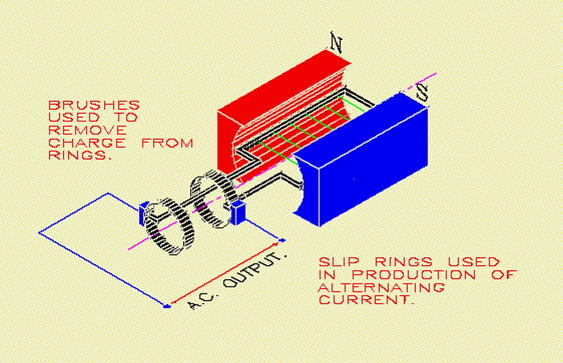
\includegraphics{aula2_9}\protect\caption{\label{fig:aula2_9}Experimento imã fixo }
\end{centering}

\end{figure}

Periodicamente, a variação de fluxo magnético na bobina (girando),
implica em uma tensão variável ao longo do tempo porque em cada hora
a bobina terá uma posição diferente (Figura \ref{fig:aula2_10}). Pela lei de Lenz a hora que injetamos
a variação de fluxo no tempo ela produz uma tensão que é contraria
ao movimento que gerou a tensão; e a posição da bobina em relação ao
campo magnético depende do tempo. Assim:

\begin{equation}\label{eq:et}
e(t)=\frac{\partial\Phi(t)}{\partial t}
\end{equation}

\begin{figure}[H]
\begin{centering}
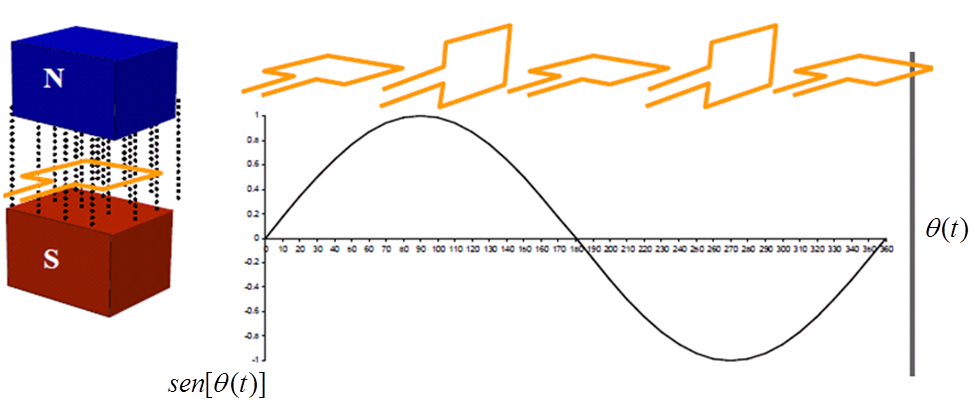
\includegraphics{aula2_10}\protect\caption{\label{fig:aula2_10}A posição da bobina }
\end{centering}

\end{figure}
Definindo $\omega$ como a velocidade angular da bobina. Pode-se escrever:

\begin{equation}\label{eq:omega}
\omega=\frac{\triangle\theta}{\triangle t}(\frac{rad}{seg})
\end{equation}

De outra forma:
\begin{equation}\label{eq:omega2}
\omega=\frac{\theta_{F}-\theta_{I}}{t_{F}-t_{I}}(\frac{rad}{seg})
\end{equation}

Considerando:

$\theta_{I}=0$ e $t_{I}=0$ então:
\begin{equation}\label{eq:omega3}
\omega=\frac{\theta_{F}}{t_{F}}=\frac{\theta}{t}
\end{equation}

Finalmente
\begin{equation}\label{eq:omega4}
\theta=\omega t
\end{equation}
A força eletromotriz $(e)$ em volts pode ser calculada como:

\begin{equation}\label{eq:ele}
e(t)=-\frac{\triangle\Phi(t)}{\triangle t}=-\frac{\partial[nBA\cos(\omega t)]}{\partial t}
\end{equation}

Assim,

$\Phi(t)=nBA\cos(\omega t)$

$e(t)=n\omega BA\sin(\omega t)$

$e(t)=E_{max}\sin(\omega t)$

$E_{max}=n\omega BA$

\begin{figure}[H]
\begin{centering}
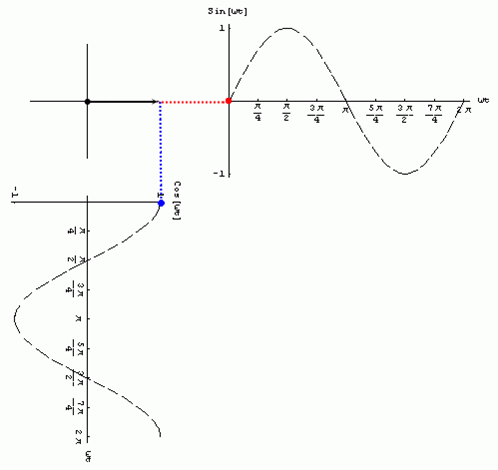
\includegraphics{aula2_11}\protect\caption{\label{fig:aula2_11}A posição da bobina }
\end{centering}

\end{figure}

Na Figura \ref{fig:aula2_11} a tensão e o fluxo variam no tempo.
Definindo $f$ como \textbf{frequência da rotação}. A frequência de rotação
descreve o numero de revoluções (voltas completas) por segundo da
bobina. Assim,

\begin{equation}\label{eq:freq}
f=\frac{n\text{º revoluções (voltas completas)}}{tempo(seg)}
\end{equation}

A unidade de frequência é hertz. Diz-se que o sistema tem um hertz
se a bobina efetua uma volta completa a cada segundo. No Brasil o
consumo em geral possui um frequência estabelecida de $60$ hertz
ou 377 radianos por segundo. 
A velocidade angular da bobina e, consequentemente, da tensão é ($2\pi$
é uma volta completa):

\begin{equation}\label{eq:omega6}
\omega=\frac{\triangle\theta}{\triangle t}(\frac{rad}{seg})
\end{equation}

De outra forma:
\begin{equation}\label{eq:omega7}
\omega=n\text{º revol.}(\frac{2\pi}{\triangle t})(\frac{rad}{seg})
\end{equation}

Então:
\begin{equation}\label{eq:omega8}
\omega=2\pi f
\end{equation}
Temos que:
\begin{equation}\label{eq:omega9}
\Phi=nBA\cos(2\pi ft)
\end{equation}

\begin{equation}\label{eq:omega10}
\ e(t)=(2\pi f)n\omega BA\sin(2\pi ft)
\end{equation}

\begin{equation}\label{eq:omega11}
[e(t)=E_{max}\sin(2\pi ft)]
\end{equation}
Trabalhar com grandezas no tempo é inconveniente no ponto de vista
matemático, então é comum mudar a forma de trabalhar com as grandezas
no setor elétrico. Como o sistema elétrico brasileiro está girando a 60 hertz,
então é tirada uma fotografia de um determinado ponto do sistema e
estabelecida
uma referencia, e ao invés de dizer que estão no domínio do tempo diz-se
que está no domínio da frequência . 
Para evitar a manipulação matemática das grandezas que variam no tempo
criou-se o conceito de fasor, um tipo especial de vetor capaz de representar
uma função sinusoidal. Isto significa que as operações com fasores
são semelhantes às de vetores.
Então a tensão no tempo varia segundo a função $f(t)=A\sin(\omega t+\theta)$.
\begin{figure}[H]
\begin{centering}
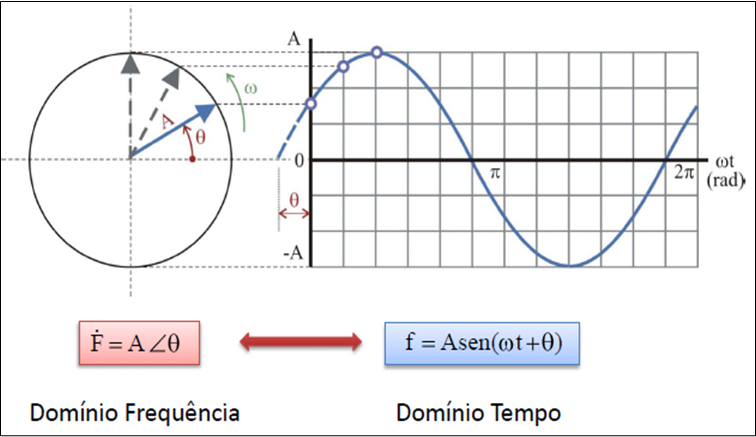
\includegraphics{aula2_12}\protect\caption{\label{fig:aula2_12}Fasores }
\end{centering}
\end{figure}
O que permite de fato levar a energia elétrica de um ponto para outro
muito distante nesse caso, aumentando a tensão é o transformador
de potencia.
O transformador de potencia é basicamente uma massa de ferro com um
enrolamento (enrola um fio em cada lado). A eficiência dos transformadores é
superior a 90\%, ou seja a energia perdida é pequena.
No transformador ideal, a tensão é gerada em função do fluxo magnético
variante no tempo, que é gerado em
função de uma corrente elétrica variante no tempo.
Se aplicarmos uma tensão de um lado, a tensão elétrica vai gerar uma
corrente que vai circular, essa corrente vai induzir um fluxo, esse
fluxo que passa no primário concatena com o secundário. Num transformador
ideal todo fluxo concatena. Quando aplicamos uma tensão, ela gera uma corrente, essa corrente vai produzir um fluxo que criará uma corrente do outro lado.
\begin{figure}[H]
\begin{centering}
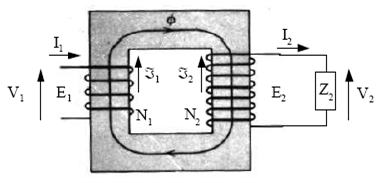
\includegraphics{aula2_13}\protect\caption{\label{fig:aula2_13}Transformador ideal de potência}
\end{centering}
\end{figure}

Matematicamente, da Lei de Faraday:
\begin{equation}\label{eq:lf}
\dot{\dot{V}_{1}=-N_{1}\frac{d\Phi}{dt}}
\end{equation}
\begin{equation}\label{eq:lf2}
\dot{\dot{V}_{2}=-N_{2}\frac{d\Phi}{dt}}
\end{equation}


onde,
$\dot{V_{i}}:$ Tensão (fasorial) no terminal i;

$\dot{I_{i}}:$ Tensão (fasorial) no terminal i;

$\dot{Ni}:$ Número de espiras no terminal i;

$\frac{d\Phi}{dt}$: Fluxo magnético variante no tempo.

Assim,

\begin{equation}\label{eq:lf2}
\frac{\dot{V}_{1}}{\dot{V}_{2}}=\frac{N_{1}}{N_{2}}=\alpha
\end{equation}

$\alpha$: Relação de transformação.

Se por exemplo colocarmos 10 espiras no primário e uma espira no secundário,eleva
a tensão no secundário para 10 vezes do primário. 
O análogo magnético (Figura \ref{fig:aula2_14}) do circuito elétrico do transformador é definido pelas equações abaixo:
\begin{equation}\label{eq:cet1}
\Im_{1}-\Im_{2}=\Re\cdot\Phi
\end{equation}

\begin{equation}\label{eq:cet2}
\Im_{1}=N_{1}\cdot\dot{I}_{1}
\end{equation}

\begin{equation}\label{eq:cet3}
\Im_{2}=N_{2}\cdot\dot{I}_{2}
\end{equation}


onde, 

$\Im_{i}$- Força magnetomotriz no terminal $i$ (A.e);

$\Phi$- Fluxo magnético induzido (Wb);

$\Re$- Relutância do transformador (A/Wb).

No transformador ideal, a relutância é nula. Assim:

\begin{equation}\label{eq:cet4}
N_{1}\cdot\dot{I}_{1}=N_{2}\cdot\dot{I}_{2}\rightarrow\frac{\dot{I}_{1}}{\dot{I}_{2}}=\frac{N_{1}}{N_{2}}=\frac{1}{\alpha}\rightarrow\dot{I}_{1}=\frac{1}{\alpha}\cdot\dot{I}_{2}
\end{equation}

\begin{figure}[H]
\begin{centering}
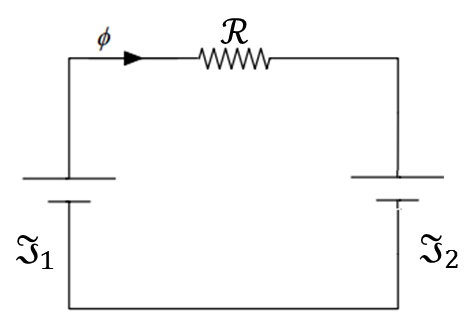
\includegraphics{aula2_14}\protect\caption{\label{fig:aula2_14}Circuito Magnético}
\end{centering}
\end{figure}

O transformador permite reduzir a corrente elétrica nas linhas
de transmissão aumentando a tensão. Neste caso, a energia elétrica
pode ser transmitida a grandes distâncias com menores perdas. 




\subsection{Evolução dos Sistemas Elétricos}


No nosso dia a dia, no trabalho, nos estudos, no lazer, sempre estamos fazendo uso da energia elétrica. A maioria das pessoas, no entanto, dão pouca importância para como esta energia chega até elas. Bom, o leite não vem da caixinha do supermercado, da mesma forma que a energia não chega magicamente às tomadas das nossas casas. Um sistema elétrico é algo muito complexo e que requer muito cuidado e planejamento. Imagine todo o Brasil interligado por uma rede de linhas de transmissão, com inúmeras unidades de geração e milhões de pessoas consumindo energia ao mesmo tempo. Quem controla tudo isso? Quem garante que a energia chegue às nossas casas? Se uma linha para de funcionar, como fazemos para levar a energia ao seu destino sem sobrecarregar demais as outras linhas?


Um sistema elétrico pode ser dividido em três partes: 1) Geração; 2) Transmissão; 3) Distribuição. A figura \ref{fig:sist} mostra um exemplo de um sistema elétrico. Tudo começa nas geradoras, que podem ser hidroelétricas, termoelétricas, torres eólicas, usinas nucleares e outras. A energia gerada vai para uma rede de transmissão básica que leva a energia até as estações de distribuição, para só então a energia chega ao consumidor final, nos famosos 110 (ou, à rigor, 127) e 220 volts que conhecemos. 

\begin{figure}[h]
\begin{centering}
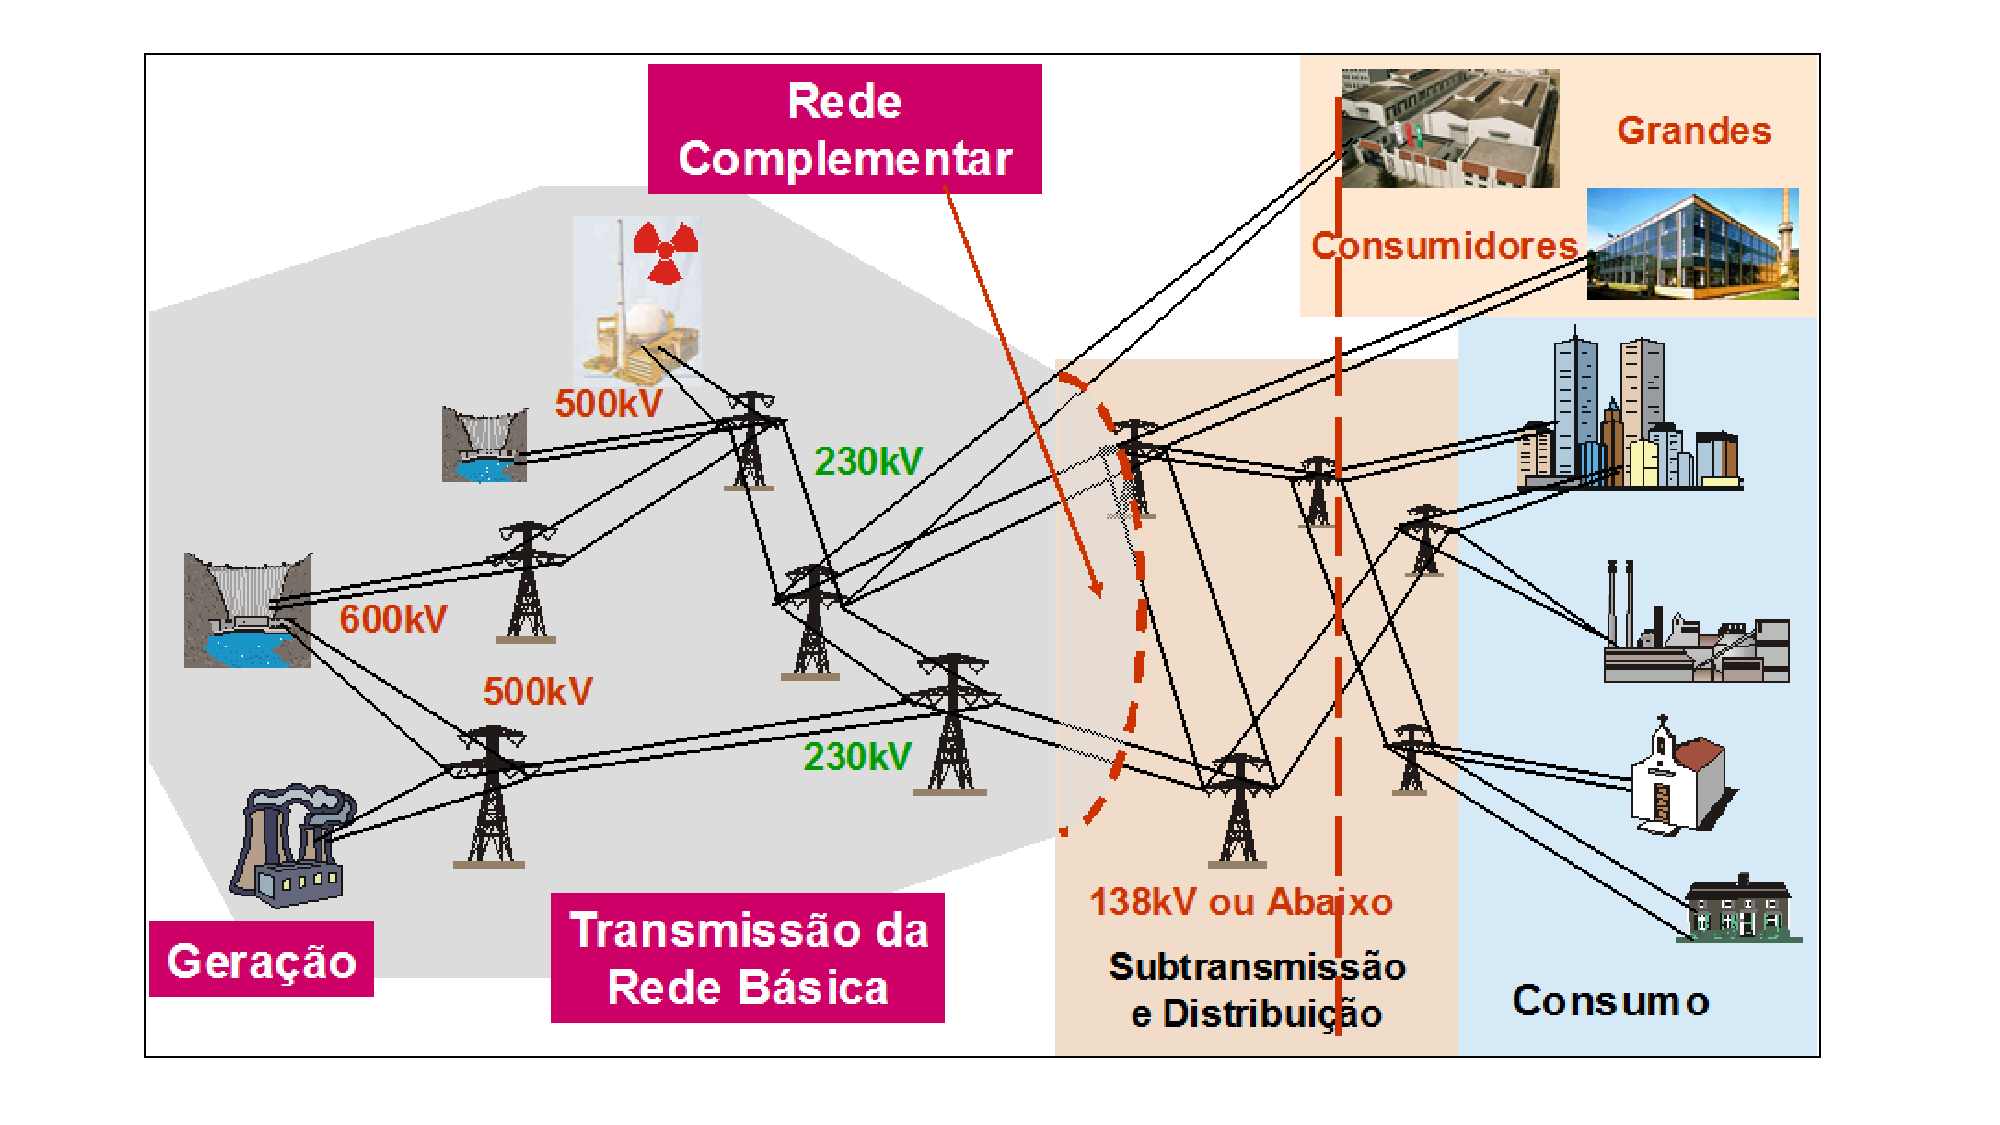
\includegraphics[scale=0.5]{anexos/figsist}
\par\end{centering}

\caption{\label{fig:sist}Representação de um sistema elétrico}
\end{figure}

\begin{figure}[h]
\begin{centering}
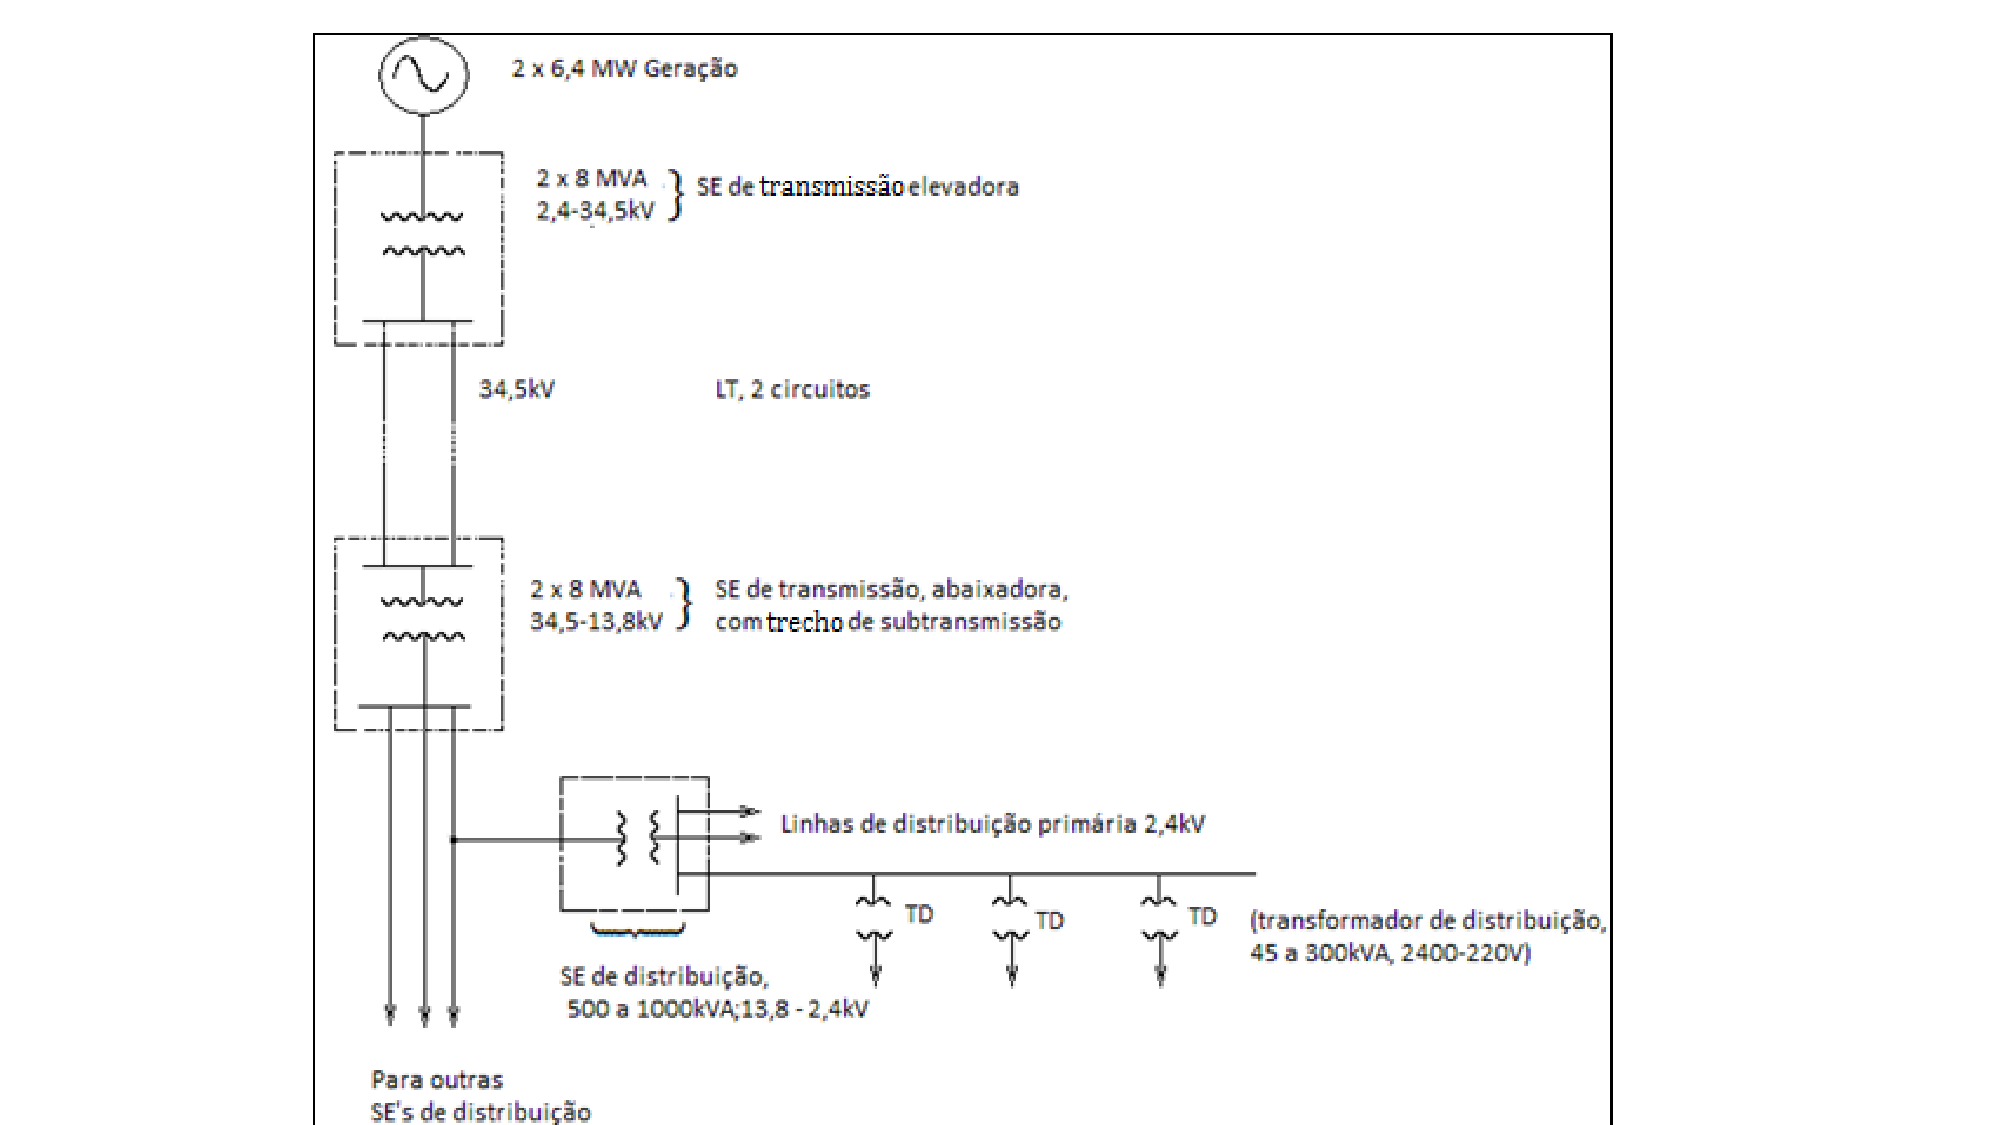
\includegraphics[scale=0.5]{anexos/figrede}
\par\end{centering}

\caption{\label{fig:rede}Sistema elétrico pequeno isolado}
\end{figure}

A figura \ref{fig:rede} mostra um pequeno sistema elétrico. As linhas e subestações no sistema são classificadas pela transformação no nível de tensão, e não a tensão no sistema como um todo. Pela figura podemos ver a tensão da geradora, que é aumentada em uma subestação. Em seguida, temos outra subestação que abaixa a tensão para 13.8kV até chegar subestação que leva às linhas de distribuição primárias, a 2.4kV. Estas linhas levam a energia até o poste, que tem um transformador que faz a energia chegar em nossas casas na tensão desejada, por exemplo, 220V. 

Já deu para notar que um sistema elétrico não é uma coisa simples, e que exige muita sincronia. Para controlar tudo isso existe o \textbf{Operador do Sistema}, que é uma entidade, que pode ou não pertencer ao governo, responsável por assegurar a funcionalidade do sistema elétrico. Dentre a funções do Operador do Sistema estão: garantir o funcionamento do mercado de energia (se ele existir), manter o sistema na frequência utilizada, assegurar que a demanda de energia será suprida, auxiliar no planejamento de expansão do sistema, minimizar custos de operação, entre outras. Estas funções podem variar de país para país.

Vamos falar agora sobre os diferentes custos de um sistema elétrico e como eles são classificados. Em primeiro lugar temos o custo de geração, que pode variar muito de gerador para gerador tanto em estrutura quando em valores absolutos. A construção de uma hidroelétrica é muito cara; entretanto, uma vez construída, a água não custa nada, ou seja, a usina não paga quase nada para funcionar. Em uma escala menor, o mesmo é valido para um parque eólico. No outro extremo estão as usinas térmicas; elas geralmente são baratas para serem construídas e podem ficar em qualquer lugar, o que reduz o custo de transmissão. No entanto, elas precisam queimar algum combustível como carvão ou gás natural, ou seja, apesar de serem baratas para construir, elas custam muito para operar. O primeiro caso que apresentamos foi o de geradores com um alto \textbf{custo fixo} e um baixo \textbf{custo variável}, no segundo caso esta relação se inverte. Além dos custos citados acima, fazem parte dos custos de geração possível custos ancilares, que podem ser custos da reserva de potência ativa, reativa, controle de frequência, controle de congestionamento do sistema, auto-restabelecimento, controle de tensão e outros.

Saindo da geração, vamos para os custos de transmissão e distribuição. Em primeiro lugar, quem arca com estes custos? Todos nós usamos linhas de transmissão, portanto o rateio destes custos pode ser algo complicado. Os custos de transmissão e distribuição são basicamente de construção e manutenção, no entanto, perdas de energia no sistema também são consideradas. É natural esperar que alguma energia será perdida no processo, e cabe ao planejador do sistema elétrico tentar minimizar estas perdas. 



\subsection{Modelagem dos Sistemas Elétricos}

Nesta seção, apresentaremos os três elementos utilizados para modelar as linhas de transmissão: resistores, indutores e capacitores. Veremos como a aplicação de uma tensão alternada se relaciona com a corrente gerada em cada um dos elementos. 

\subsubsection*{Resistores}


\begin{figure}
    \centering
    \begin{subfigure}[b]{0.3\textwidth}
        \centering
        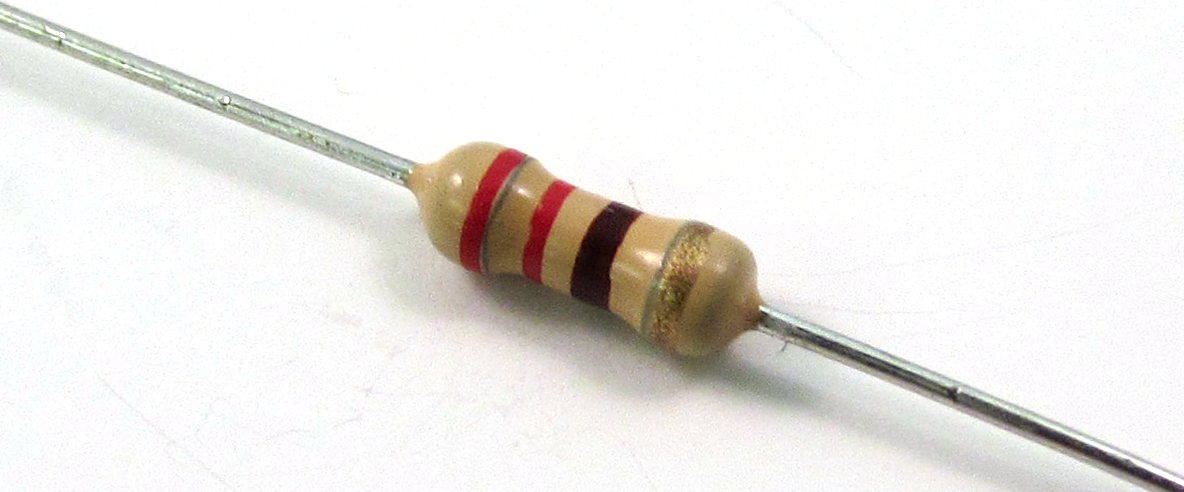
\includegraphics[width=\textwidth]{anexos/resistor.png}
        %\caption{$y=x$}
        %\label{fig:y equals x}
    \end{subfigure}
    \hspace{1cm}
    \begin{subfigure}[b]{0.3\textwidth}
        \centering
        \fbox{
            \begin{circuitikz} \draw
            (0,0) to[R, o-o, l=R] (0,2.5)
            ;
            \end{circuitikz}%\caption{$y=3sinx$}
            }
        %\label{fig:three sin x}
    \end{subfigure}
    

    \caption{À esquerda, um resistor real. À direita, a representação esquemática de um resistor.}
    \label{fig:three graphs}
\end{figure}


São equipamentos com características resistivas, como chuveiro elétrico
e aquecedor. As equações para a tensão ($V$) e corrente ($i$) em
função do tempo, assim como a representação com seus fasores correspondentes,
são exibidas a seguir:

\[
i(t)=\frac{V_{m}}{R}\mbox{\, sen}(wt+\phi)\qquad\longrightarrow\qquad\dot{I}=\frac{V_{m}}{R}\angle\phi^{\circ},
\]


\[
V(t)=V_{m}\mbox{\, sen}(wt+\phi)\qquad\longrightarrow\qquad\dot{V}=V_{m}\angle\phi^{\circ},
\]
em que $V_{m}$ é o valor máximo da tensão, ou seja, a sua amplitude.
A notação de fasor é uma forma simplificada de determinar a grandeza
no tempo, sem ter que especificar a função no sentido temporal, desde
que a frequência seja a mesma para todas as funções. No sistema elétrico utiliza-se comumente
frequências entre 50 e 60Hz. No Brasil, o padrão é de 60Hz. 

Para um resistor tem-se no domínio do tempo que 
\[
V(t)/i(t)=\frac{\frac{V_{m}}{R}\mbox{\, sen}(wt+\phi)}{V_{m}\mbox{\, sen}(wt+\phi)}=R
\]
 e no domínio da frequência que 
\[
\dot{V}/\dot{I}=R.
\]
 Assim, a fase que a corrente se encontra é exatamente a mesma da
tensão, como mostra a figura \ref{fig:fase-ct-resistor}. Como será
visto a seguir, isto não acontece para indutores e capacitores.



%\begin{center}
%\begin{table}[H]
%\begin{tabular}{ll}
%\multirow{2}{5cm}{  \begin{circuitikz} \draw
%    (0,0) to[R, o-o, l=R] (0,3)
%    ;
%    \end{circuitikz}}    & $e = E_m\text{sen}(wt+\phi)$ \\
%                                        & $i=\dfrac{E_m}{R}\text{sen}(wt+\phi)$ \\
%\end{tabular}
%\end{table}
%\end{center}

%\begin{figure}[H]
%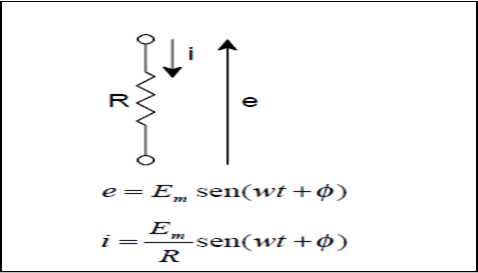
\includegraphics{anexos/aula2_1.png}\protect\caption{Resistores}
%\end{figure}




%Figura resistor
\begin{figure}[H]
\begin{center}
\fbox {
    \begin{tikzpicture}[domain=0:4]
        \draw[very thin,color=gray] (-0.1,-2.1) grid (3.9,2.1);
        \draw[->] (-0.2,0) -- (4.2,0) node[right] {$t$};
        \draw[->] (0,-2.2) -- (0,2.2) node[above] {};
        \draw[smooth, color=blue] plot[id=sin] function{sin(5*x)} 
            node[right] {$i(t)=\frac{V_{m}}{R}\mbox{\,\ sen}(wt+\phi)$};
        \draw[smooth, color=orange] plot[id=exp] function{2*sin(5*x)} 
            node[right] {$V=V_{m}\mbox{\, sen}(wt+\phi)$};
    \end{tikzpicture}
    }
\caption{\label{fig:fase-ct-resistor}Corrente e tensão oscilam na mesma fase no resistor}
\end{center}
\end{figure}


\subsubsection*{Indutores}

% Figura Indutor
\begin{figure}
    \centering
    \begin{subfigure}[b]{0.3\textwidth}
        \centering
        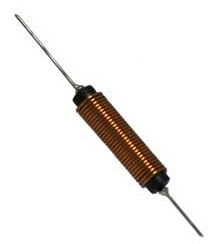
\includegraphics[width=\textwidth]{anexos/indutor.png}
        %\caption{$y=x$}
        %\label{fig:y equals x}
    \end{subfigure}
    \hspace{1cm}
    \begin{subfigure}[b]{0.3\textwidth}
        \centering
        \fbox{
            \begin{circuitikz} \draw
            (0,0) to[cute inductor, o-o, l=L] (0,2.5)
            ;
            \end{circuitikz}%\caption{$y=3sinx$}
            }
        %\label{fig:three sin x}
    \end{subfigure}
    \caption{À esquerda, um indutor real. À direita, a representação esquemática de um indutor.}
    \label{fig:three graphs}
\end{figure}


Quando a corrente passa por equipamentos como um motor elétrico ou
um transformador (elementos indutivos), a fase da corrente se atrasa
com relação à tensão. Sendo a diferença de potencial num indutor medido
como $V=L\,\frac{di}{dt}$, em que $L$ é a indutância, apresentamos a seguir o cálculo das relações
entre corrente e tensão a seguir:

\[
i(t)=\frac{V_{m}}{R}\mbox{\,\ sen}(wt+\phi)\qquad\longrightarrow\qquad\dot{I}=I_{m}\angle\phi^{\circ},
\]


\[
V(t)=L\,\frac{di}{dt}=wLI_{m}\mbox{cos}(wt+\phi)=wLI_{m}\mbox{sen}(wt+\phi+90)\qquad\longrightarrow\qquad\dot{V}=wLI_{m}\angle\phi+90^{\circ},
\]


\begin{equation}
\frac{\dot{V}}{\dot{I}}=\frac{wLI_{m}\angle\phi+90^{\circ}}{I_{m}\angle\phi^{\circ}}=wL\angle90^{\circ}.\label{eq:fase-v-i}
\end{equation}
Assim, conforme visto nas equações acima, a fase da corrente num indutor
se atrasa em $90^{\circ}$ com relação à tensão. A forma regular da
expressão \ref{eq:fase-v-i} pode ser escrita também como um número
complexo num plano de Argand-Gauss: 
\[
\frac{\dot{V}}{\dot{I}}=jwL.
\]
Este plano é similar ao plano cartesiano, com a diferença que no eixo horizontal está a parte real $a$ do número $a+bj$ e no eixo vertical a parte imaginária $b.$ Nota-se que utiliza-se a letra $j$ para representar $\sqrt{-1}$, pois a letra $i$ já é usada para denominar a corrente. Denomina-se como \textbf{reatância indutiva} ($X_L$)o valor equivalente de resistência que o indutor provoca no sistema. 



% Figura senoide Indutor
\begin{figure}[H]
\begin{center}
\fbox {
    \begin{tikzpicture}[domain=0:4]
        \draw[very thin,color=gray] (-0.1,-2.1) grid (3.9,2.1);
        \draw[->] (-0.2,0) -- (4.2,0) node[right] {$t$};
        \draw[->] (0,-2.2) -- (0,2.2) node[above] {};
        \draw[smooth, color=blue] plot[id=sin] function{sin(6*x)} 
            node[right] {$\dot{I}=I_{m}\angle\phi^{\circ}$};
        \draw[smooth, color=orange] plot[id=exp] function{2*sin(6*x+90)} 
            node[right] {$\dot{V}=wLI_{m}\angle\phi+90^{\circ}$};
    \end{tikzpicture}
    }
\caption{\label{fig:fase-ct-indutor}Corrente é atrasada em 90º com relação à tensão num indutor}
\end{center}
\end{figure}


\subsubsection*{Capacitores}

%Figura capacitor 
\begin{figure}
    \centering
    \begin{subfigure}[b]{0.3\textwidth}
        \centering
        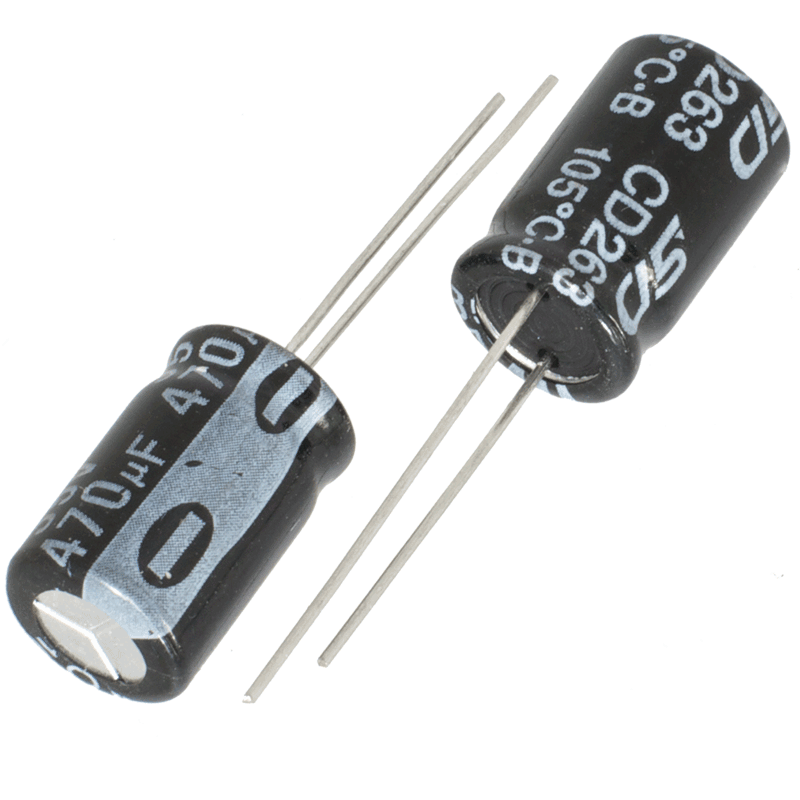
\includegraphics[width=\textwidth]{anexos/capacitor.png}
        %\caption{$y=x$}
        %\label{fig:y equals x}
    \end{subfigure}
    \hspace{1cm}
    \begin{subfigure}[b]{0.3\textwidth}
        \centering
        \fbox{
            \begin{circuitikz} \draw
            (0,0) to[capacitor, o-o, l=C] (0,2.5)
            ;
            \end{circuitikz}%\caption{$y=3sinx$}
            }
        %\label{fig:three sin x}
    \end{subfigure}
    \caption{À esquerda, um resistor real. À direita, a representação esquemática de um resistor.}
    \label{fig:three graphs}
\end{figure}


O único elemento capacitivo numa rede são os próprios bancos de capacitores.
Ele é utilizado principalmente para regulagem da tensão e fator de
potência. Sendo $C$ a capacitância do capacitor em questão, temos
que:

\[
V(t)=V_{m}\mbox{\,\ sen}(wt+\phi)\qquad\longrightarrow\qquad\dot{V}=V_{m}\angle\phi^{\circ},
\]


\[
i(t)=C\,\frac{dV}{dt}=wCV_{m}\mbox{cos}(wt+\phi)=wCV_{m}\,\mbox{sen}(wt+\phi+90)\qquad\longrightarrow\qquad\dot{I}=wCV_{m}\angle\phi+90^{\circ},
\]


\[
\frac{\dot{V}}{\dot{I}}=\frac{V_{m}\angle\phi^{\circ}}{wCV_{m}\angle\phi+90^{\circ}}=\frac{1}{wC\angle90^{\circ}}.
\]
Passando para a forma retangular através de números complexos, temos que
\[
\frac{\dot{V}}{\dot{I}}=\frac{1}{jwC}=\frac{-j}{wC}.
\]
Assim, a reatância capacitiva é dada por $X_{C}=\frac{1}{wC}$. 

% Figura capacitor
\begin{figure}[H]
\begin{center}
\fbox {
    \begin{tikzpicture}[domain=0:4]
        \draw[very thin,color=gray] (-0.1,-2.1) grid (3.9,2.1);
        \draw[->] (-0.2,0) -- (4.2,0) node[right] {$t$};
        \draw[->] (0,-2.2) -- (0,2.2) node[above] {};
        \draw[smooth, color=blue] plot[id=sin] function{sin(5*x)} 
            node[right] {$\dot{I}=I_{m}\angle\phi^{\circ}$};
        \draw[smooth, color=orange] plot[id=exp] function{2*sin(5*x-90)} 
            node[right] {$\dot{V}=wLI_{m}\angle\phi+90^{\circ}$};
    \end{tikzpicture}
    }
\caption{\label{fig:fase-ct-indutor}Corrente é adiantada em 90º com relação à tensão num capacitor}
\end{center}
\end{figure}

\subsubsection*{Linhas de transmissão}

Para modelar as linhas de transmissão, verifica-se qual a impedância do sistema. A impedância é dada pela combinação da resistência, reatância capacitiva e reatância indutiva.

% Figura corrente alternada
%\begin{figure}[H]
%\begin{center}
%\fbox {
%    \begin{tikzpicture}[domain=0:4]
%        \draw[very thin,color=gray] (-0.1,-2.1) grid (3.9,2.1);
%        \draw[->] (-0.2,0) -- (4.2,0) node[right] {$t$};
%        \draw[->] (0,-2.2) -- (0,2.2) node[above] {$V$};
%        \draw[smooth, color=blue] plot[id=sin] function{sin(5*x)} 
%            node[right] {Corrente alternada};
%    \end{tikzpicture}
%    }
%\caption{\label{fig:fase-ct-indutor}Corrente é atrasada em 90º com relação à tensão num indutor}
%\end{center}
%\end{figure}
%
%
%
%
%% Figura corrente contínua
%\begin{figure}[H]
%\begin{center}
%\fbox {
%    \begin{tikzpicture}[domain=0:4]
%        \draw[very thin,color=gray] (-0.1,-0.1) grid (3.9,3.9);
%        \draw[->] (-0.2,0) -- (4.2,0) node[right] {$i$};
%        \draw[->] (0,-0.2) -- (0,4.2) node[above] {$V$};
%        \draw[smooth, color=blue] plot[id=sin] function{2} 
%            node[right] {Corrente contínua};
%    \end{tikzpicture}
%    }
%\caption{\label{fig:fase-ct-indutor}Corrente é atrasada em 90º com relação à tensão num indutor}
%\end{center}
%\end{figure}
%
%
%
%\begin{center}
%\begin{tikzpicture}
%    \begin{axis}[domain=0:1,legend pos=outer north east]
%    \addplot[smooth] {2*sin(20*deg(x))}; 
%    \addplot[smooth, red] {sin(20*deg(x))}; 
%    \legend{$i=\frac{E_{m}}{R}\mbox{\,\ sen}(wt+\phi)$,$
%e=E_{m}\mbox{\, sen}(wt+\phi)$}
%    \end{axis}
%\end{tikzpicture}
%\end{center}


%\bibliographystyle{apalike}
%\bibliography{bib_apostila}

\end{document}